%==========================================================%
\newif\ifdraft
\newif\iffull
\newif\ifcomment
\newif\iflatexdiff
\newif\ifbibtex
\newif\ifpreprint
\latexdifftrue   %enable latex diff commands
\drafttrue       %enable draft banner and version number
\bibtextrue      %enable bibtex (off for final preprint or paper)
\preprinttrue    %enable cern preprint (for arXiv)
%\fulltrue        %include author and acknowledgement and references (refpaper.tex/refpreprint.tex)
% paper style defintions
\newif\ifplbpaper
\newif\ifapspaper
\apspapertrue
%
\def\snntitle{$\snn$}
\ifpreprint
\def\snntitle{$\snnbf$}
\fi
\def\dvers{v0.0}       % Set version number by hand every time you want to change it
\def\dtitle{$\Lambda$ and \ks in jets in \pPb collisions at \sqrtsnn{5.02}}
\def\stitle{$\Lambda$ and \ks in jets} % Put a short paper title (only relevant for CERN paper)
\def\phnum{2015-XXX}     % Required, obtained from PH
\def\phdat{xx yyy 2015}  % Required, obtained from PH
%%\def\bibstname{utphys}   % Put here the style file name for the paper
\def\bibstname{./LaTeX/utphys}   % Put here the style file name for the paper
\def\revision{rev. 0}

%==========================================================%
\ifpreprint
\documentclass[ALICE,manyauthors,12pt]{LaTeX/cernphprep}
\usepackage[comma,square,numbers,sort&compress]{natbib}
\usepackage{booktabs}
\else %%% PUT PAPER STYLE BELOW %%%
\ifplbpaper
\documentclass[final,3p,12pt]{elsarticle}
\biboptions{comma,square,numbers,sort&compress}
\def\bibstname{utphys}
\fi
\ifapspaper
\documentclass[10pt,aps,prl,superscriptaddress,altaffilletter,nobibnotes,nofootinbib]{revtex4-1}
\newenvironment{frontmatter}{}{\maketitle}
\def\bibstname{apsrev4-1}
\fi
\fi
%==========================================================%
% Remove any % below to load the required packages
\usepackage{graphicx}  % needed for figures
\usepackage{dcolumn}   % needed for some tables
\usepackage{bm}        % for math
\usepackage{amssymb}   % for math
\usepackage{amsfonts}
\usepackage{graphics}
\usepackage{grffile}   % to handle dots in graphics file names
\usepackage{epsfig}
\usepackage{units}
\usepackage{hyperref}
\usepackage[usenames]{color}
\usepackage[normalem]{ulem} % for strikethroughs (\sout{})
\usepackage{color}
\usepackage[utf8]{inputenc}
\usepackage[T1]{fontenc}
\usepackage{array}
\usepackage{multirow}
\usepackage{float}

\newcolumntype{P}[1]{>{\centering\arraybackslash}p{#1}}
\newcolumntype{M}[1]{>{\centering\arraybackslash}m{#1}}
\iflatexdiff
\RequirePackage{color}\definecolor{RED}{rgb}{1,0,0}\definecolor{BLUE}{rgb}{0,0,1}
\providecommand{\DIFadd}[1]{{\protect\color{blue}\uwave{#1}}}
\providecommand{\DIFdel}[1]{{\protect\color{red}\sout{#1}}}
\providecommand{\DIFaddbegin}{}
\providecommand{\DIFaddend}{}
\providecommand{\DIFdelbegin}{}
\providecommand{\DIFdelend}{}
\providecommand{\DIFaddFL}[1]{\DIFadd{#1}}
\providecommand{\DIFdelFL}[1]{\DIFdel{#1}}
\providecommand{\DIFaddbeginFL}{}
\providecommand{\DIFaddendFL}{}
\providecommand{\DIFdelbeginFL}{}
\providecommand{\DIFdelendFL}{}
\fi
%==========================================================%
%!TEX root = ../AliPubV0JetspPb.tex

\newcommand{\ev}           {\ensuremath{\mathrm{eV}}} 
\newcommand{\kev}          {\ensuremath{\mathrm{keV}}}  
\newcommand{\mev}          {\ensuremath{\mathrm{MeV}}}
\newcommand{\mevc}         {\ensuremath{\mathrm{MeV}/c}}    
\newcommand{\mevcc}        {\ensuremath{\mathrm{MeV}/c^2}}     
\newcommand{\gev}          {\ensuremath{\mathrm{GeV}}}  
\newcommand{\gevc}         {\ensuremath{\mathrm{GeV}/c}}    
\newcommand{\GeVc}         {\ensuremath{\mathrm{GeV}/c}}    
\newcommand{\gevcc}        {\ensuremath{\mathrm{GeV}/c^{2}}}    
\newcommand{\tev}          {\ensuremath{\mathrm{TeV}}}  
\newcommand{\tevc}         {\ensuremath{\mathrm{TeV}/c}}    

\newcommand{\etal}         {\ensuremath{\eta_{\mathrm{lab}}}}
\newcommand{\dNdetal}      {\mathrm{d}N_\mathrm{ch}/\mathrm{d}\etal}
\newcommand{\dNdetatrl}    {\mathrm{d}N_\mathrm{tracklets}/\mathrm{d}\etal}
\newcommand{\dNdetarl}[1]  {\mathrm{d}N_\mathrm{ch}/\mathrm{d}\etal\left.\right|_{|\etal|<#1}}
\newcommand{\etac}         {\ensuremath{\eta_{\mathrm{cms}}}}
\newcommand{\dNdetac}      {\mathrm{d}N_\mathrm{ch}/\mathrm{d}\etac}
\newcommand{\dNdetatrc}    {\mathrm{d}N_\mathrm{tracklets}/\mathrm{d}\etac}
\newcommand{\dNdetarc}[1]  {\mathrm{d}N_\mathrm{ch}/\mathrm{d}\etal\left.\right|_{|\etac|<#1}}
\newcommand{\vn}           {\ensuremath{v_{n}}}
\newcommand{\vngf}         {\ensuremath{v_{n} \{ GF \} }}
\newcommand{\vnd}          {\ensuremath{V_{n\Delta}}}
\newcommand{\voned}        {\ensuremath{V_{1\Delta}}}
\newcommand{\ptt}          {\ensuremath{p_{\mathrm{T, trig}}}}
\newcommand{\pta}          {\ensuremath{p_{\mathrm{T, assoc}}}}
\newcommand{\CF}           {\ensuremath{C \left(\Delta \phi \right)}}
\newcommand{\same}         {\ensuremath{frac{d\langle n_{\mathrm{same}}^{AB} \rangle}{d\Delta\phi}}}
\newcommand{\mix}          {\ensuremath{frac{d\langle n_{\mathrm{mix}}^{AB} \rangle}{d\Delta\phi}}}
\newcommand{\ITS}          {\rm{ITS}}
\newcommand{\TOF}          {\rm{TOF}}
\newcommand{\ZNA}          {\rm{ZNA}}
\newcommand{\ZNC}          {\rm{ZNC}}
\newcommand{\ZDC}          {\rm{ZDC}}
\newcommand{\ZDCs}         {\rm{ZDCs}}
\newcommand{\SPD}          {\rm{SPD}}
\newcommand{\SDD}          {\rm{SDD}}
\newcommand{\SSD}          {\rm{SSD}}
\newcommand{\TPC}          {\rm{TPC}}
\newcommand{\VZERO}        {\rm{VZERO}}
\newcommand{\VZEROA}       {\rm{VZERO-A}}
\newcommand{\VZEROC}       {\rm{VZERO-C}}
\newcommand{\dg}           {\mbox{$^\circ$}}
\newcommand{\pp}           {\text{pp}}
\newcommand{\ppbar}        {\mbox{$\mathrm{p\overline{p}}$}}
\newcommand{\mpp}          {\mathrm{pp}}
\newcommand{\PbPb}         {\mbox{Pb--Pb}}
\newcommand{\AuAu}         {\mbox{Au--Au}}
\newcommand{\pPb}          {\mbox{p--Pb}}
\newcommand{\pA}           {\mbox{p--A}}
\newcommand{\Pbp}          {\mbox{Pb--p}}
\newcommand{\dAu}          {\mbox{d--Au}}
\newcommand{\pAu}          {\mbox{p--Au}}
\newcommand{\pseudorap}    {\mbox{$\left | \eta \right | $}}
\newcommand{\lum}          {\, \mbox{${\mathrm{cm}}^{-2} {\mathrm{s}}^{-1}$}}
\newcommand{\barn}         {\, \mbox{${\mathrm{barn}}$}}
\newcommand{\m}            {\, \mbox{${\mathrm{m}}$}}
\newcommand{\pt}           {\ensuremath{p_{\mathrm{T}}}}
\newcommand{\ptjet}        {\ensuremath{p_{\mathrm{T}}^{\mathrm{jet}}}}
\newcommand{\pT}           {\ensuremath{p_{\mathrm{T}}}}
\newcommand{\mt}           {\ensuremath{m_{\mathrm{t}}}}
\newcommand{\snn}          {\ensuremath{\sqrt{s_{\mathrm{NN}}}}}
\newcommand{\sqrtsnn}[1]   {\ensuremath{\sqrt{s_{\mathrm{NN}}}=#1~\mathrm{TeV}}}
\newcommand{\sqrts}[1]     {\ensuremath{\sqrt{s}=#1~\mathrm{TeV}}}
\newcommand{\sqts}         {\sqrt{s}}
\newcommand{\snnbf}        {\ensuremath{\mathbf{{\sqrt{s_{\mathbf NN}}}}}}
\newcommand{\sonly}        {\ensuremath{\sqrt{s}}}
\newcommand{\Npart}        {\ensuremath{N_\mathrm{part}}}
\newcommand{\avNpart}      {\ensuremath{\langle N_\mathrm{part} \rangle}}
\newcommand{\avNpartdata}  {\ensuremath{\langle N_\mathrm{part}^{\mathrm{data}} \rangle}}
\newcommand{\Ncoll}        {\ensuremath{N_\mathrm{coll}}}
\newcommand{\Dnpart}       {\ensuremath{D\left(\Npart\right)}}
\newcommand{\DnpartExp}    {\ensuremath{D_{\mathrm{exp}}\left(\Npart\right)}}
\newcommand{\abs}[1]       {\ensuremath{\left|#1\right|}}
\newcommand{\avg}[1]       {\ensuremath{\left\langle#1\right\rangle}}
\newcommand{\signn}        {\ensuremath{\sigma^{\mathrm{inel.}}_{\mathrm{NN}}}}
\newcommand{\vz}           {\ensuremath{V_{z}}}
\newcommand{\dd}           {\ensuremath{\mathrm{d}}}
\newcommand{\ade}          {\ensuremath{\abs{\Delta\eta}}}
\newcommand{\Dphi}         {\ensuremath{\Delta\varphi}}
\newcommand{\Deta}         {\ensuremath{\Delta\eta}}
\newcommand{\Ntrig}        {\ensuremath{N_{\mathrm{trig}}}}
\newcommand{\Nassoc}       {\ensuremath{N_{\mathrm{assoc}}}}
\newcommand{\dNassoc}      {\ensuremath{\frac{\dd^2N_{\mathrm{assoc}}}{\dd\Deta\dd\Dphi}}}
\newcommand{\stat}         {({\it stat.})}
\newcommand{\syst}         {({\it sys.})}
\newcommand{\Fig}[1]       {Fig.~\ref{#1}}
\newcommand{\Figure}[1]    {Figure~\ref{#1}}
\newcommand{\Sect}[1]      {Sect.~\ref{#1}}
\newcommand{\Section}[1]   {Section~\ref{#1}}
\newcommand{\Sections}[1]  {Sections~\ref{#1}}
\newcommand{\Eq}[1]        {Eq.~\ref{#1}}
\newcommand{\Equation}[1]  {Equation~\ref{#1}}
\newcommand{\Ref}[1]       {Ref.~\cite{#1}}
\newcommand{\Refs}[1]      {Refs.~\cite{#1}}
\newcommand{\green}[1]     {\textcolor{green}{#1}}
\newcommand{\blue}[1]      {\textcolor{blue}{#1}}
\newcommand{\red}[1]       {\textcolor{red}{#1}}
\newcommand{\white}[1]     {\textcolor{white}{#1}}
\newcommand{\warn}[1]      {{\small\textbf{\red{(!}\footnote{\textbf{\red{(!)}}~#1}\red{)}}}\marginpar{\textbf{\red{---}}}}
\newcommand{\todo}[1]      {{\textcolor{red}{TODO: #1}}}
\newcommand{\high}[1]      {{\textcolor{blue}{#1}}}
\newcommand{\fake}[1]      {{\textcolor{red}{#1}}}
\newcommand{\final}[1]     {{\textcolor{blue}{#1}}}
\newcommand{\prelim}[1]    {{\textcolor{magenta}{#1}}}
\newcommand{\orig}[1]      {{\textcolor{red}{\sout{#1}}}}
\newcommand{\repl}[1]      {{\textcolor{blue}{#1}}}
\newcommand*{\doi}[1]      {\href{http://dx.doi.org/#1}{doi: #1}}
\newcommand{\arxiv}[1]     {\href{http://www.arxiv.org/abs/#1}{\mbox{arXiv:#1}}}
\newcommand{\com}[1]       {}
\newcommand{\expval}[1]    {\langle #1 \rangle}
\newcommand{\RAA}          {\ensuremath{R_{\mathrm{AA}}}}
\newcommand{\Journal}[1]   {{\bf{#1}}}
\newcommand{\PRC}          {Phys.~Rev.~C~}
\newcommand{\PLB}          {Phys.~Lett.~B~}

\iflatexdiff
\newcommand{\blu}[1]       {\textcolor{blue}{#1}}
\renewcommand{\xout}[1]    {\textcolor{red}{\sout{#1}}}
\newcommand{\ask}[1]       {\textcolor{magenta} {#1} } 
\else
\newcommand{\blu}[1]       {#1}
\renewcommand{\xout}[1]    {}
\newcommand{\ask}[1]       {}
\fi

\newcommand{\av}[1]        {\left\langle #1 \right\rangle}
\newcommand{\lsim}         {\,{\buildrel < \over {_\sim}}\,}
\newcommand{\gsim}         {\,{\buildrel > \over {_\sim}}\,}
\newcommand{\fm}           {\mathrm{fm}}
\newcommand{\mm}           {\mathrm{mm}} 
\newcommand{\cm}           {\mathrm{cm}}
%%\newcommand{\m}          {\mathrm{m}}
\newcommand{\mum}          {\mathrm{\mu m}}
\newcommand{\secs}         {\mathrm{s}}
\newcommand{\ns}           {\mathrm{ns}}
\newcommand{\mrad}         {\mathrm{mrad}}
\newcommand{\mb}           {\mathrm{mb}}
\newcommand{\mub}          {\mathrm{\mu b}}
\newcommand{\T}            {\mathrm{T}}
\newcommand{\dNdy}         {{\rm d}N_{ch}/{\rm d}y}
\newcommand{\momwin}       {[$p$, $p$+$\Delta$ $p$]}
\newcommand{\DtoKpi}       {{\rm D}^0 \to {\rm K}^-\pi^+}
\newcommand{\DtoKpipi}     {{\rm D}^+\to {\rm K}^-\pi^+\pi^+}
\newcommand{\DstartoDpi}   {{\rm D}^{*+} \to {\rm D}^0 \pi^+}
\newcommand{\Dzero}        {{\rm D^0}}
\newcommand{\Dzerobar}     {\overline{{\rm D^0}}}
\newcommand{\Dstar}        {{\rm D^{*+}}}
\newcommand{\Dstarm}       {{\rm D^{*-}}}
\newcommand{\Dplus}        {{\rm D^+}}
\newcommand{\Dminus}       {{\rm D^-}}
\newcommand{\Ds}           {{\rm D^+_{\rm s}}}
\newcommand{\Lc}           {{\rm \Lambda^+_{\rm c}}}
\newcommand{\ccbar}        {${\rm c}\bar{\rm c}$~}
\newcommand{\bbbar}        {${\rm b}\bar{\rm b}$~}
\newcommand{\nbinv}        {{\rm nb^{-1}}}
\newcommand{\decleng}      {{\rm L}_{xyz}}
\newcommand{\cubar}        {{\rm c}\bar{\rm u}}
\newcommand{\cdbar}        {{\rm c}\bar{\rm d}}
\newcommand{\mur}          {\mu_{\rm R}}
\newcommand{\muf}          {\mu_{\rm F}}
\newcommand{\mc}           {m_{\rm c}}
\newcommand{\sigmatot}     {\sigma_{\rm tot}}
\newcommand{\Ntrk}         {N_{\rm tracklets}}
\newcommand{\Nvzero}       {N_{\rm V0}}
\newcommand{\fB}           {f_{\rm B}}

\newcommand{\pip}          {\ensuremath{\pi^{+}}}
\newcommand{\pim}          {\ensuremath{\pi^{-}}}
\newcommand{\kap}          {\ensuremath{\rm{K}^{+}}}
\newcommand{\kam}          {\ensuremath{\rm{K}^{-}}}
\newcommand{\pbar}         {\ensuremath{\overline{\rm p}}}
\newcommand{\degree}       {\ensuremath{^{\rm o}}}
\newcommand{\dedx}         {\ensuremath{{\rm d}E/{\rm d}x}}
\newcommand{\jpsi}         {\ensuremath{{\rm J}/\psi}}
\newcommand{\psip}         {\ensuremath{\psi^{\prime}}}
\newcommand{\jpsiDY}       {\rm J/$\psi$\,/\,DY}
\newcommand{\chic}         {\ensuremath{\chi_{\rm c}}}
\newcommand{\ezdc}         {\ensuremath{E_{\rm ZDC}}}
\newcommand{\slfrac}[2]    {\left.#1\right/#2}
\newcommand{\dndydpT}      {\ensuremath{{\rm d}^{2}N/{\rm d}y{\rm d}p_{\rm T}}}
\newcommand{\Kshort}       {\ensuremath{{\rm K}_{\rm S}^{0}}}
\newcommand{\ks}           {\ensuremath{\rm{K}^{0}_{\rm S}}}
\newcommand{\lda}     	   {\ensuremath{\Lambda}}
\newcommand{\alda}         {\ensuremath{\overline{\Lambda}}}
\newcommand{\AntiLa}       {\ensuremath{\overline{\Lambda}}}
\newcommand{\Vzero}        {\ensuremath{{\rm V}^{0}}}
\newcommand{\Vzeros}       {\ensuremath{{\rm V}^{0}{\rm s}}}
\newcommand{\kT}           {\ensuremath{k_{\rm T}}}
\newcommand{\akT}           {\ensuremath{{\rm anti-}k_{\rm T}}}

\newcommand{\dNdetapt}     {\ensuremath{\dNdeta\,/\left(0.5\Npart\right)}}
\newcommand{\dNdetaptr}[1] {\ensuremath{\dNdetar{#1}\,/\left(0.5\Npart\right)}}
\newcommand{\dNdetape}     {\ensuremath{\left(\dNdeta\right)/\left(\avNpart/2\right)}}
\newcommand{\dNdetaper}[1] {\ensuremath{\dNdetar{#1}\,/\left(\avNpart/2\right)}}
\newcommand{\dndy}         {\ensuremath{{\mathrm{d}N/{\mathrm{d}y}}}}
\newcommand{\dndydpt}      {\ensuremath{{\mathrm{d}}^2N/({\mathrm{d}}y {\mathrm{d}}\pt)}}
\newcommand{\dNdeta}       {\mathrm{d}N_\mathrm{ch}/\mathrm{d}\eta}
\newcommand{\dNdetatr}     {\mathrm{d}N_\mathrm{tracklets}/\mathrm{d}\eta}
\newcommand{\dNdetar}[1]   {\mathrm{d}N_\mathrm{ch}/\mathrm{d}\eta\left.\right|_{|\eta|<#1}}
\newcommand{\dNdEta}       {{\rm d}N_{\rm ch}/{\rm d}\eta}

\newcommand{\bT}           {\ensuremath{\beta_{\rm T}}}
\newcommand{\avbT}         {\ensuremath{\left< \beta_{\rm T}\right>}}
\newcommand{\avpT}         {\ensuremath{\left< \pt \right>}}
\newcommand{\muB}          {\ensuremath{\mu_{B}}}
\newcommand{\kzero}        {\ensuremath{{\rm K}^{0}_{S}}}
\newcommand{\vzero}        {\ensuremath{{\rm V}^0}}
\newcommand{\lmb}          {\ensuremath{\Lambda}}
\newcommand{\almb}         {\ensuremath{\bar{\Lambda}}}
\newcommand{\Tfo}          {\ensuremath{{T}_{\rm kin}}}
\newcommand{\Tch}          {\ensuremath{{T}_{\rm ch}}}
\newcommand{\hlab}         {\ensuremath{\eta_{\rm lab}}}
\newcommand{\ynn}         {\ensuremath{y_{\rm NN}}}
\newcommand{\ycms}         {\ensuremath{y_{\rm CMS}}}
\newcommand{\ylab}         {\ensuremath{y_{\rm lab}}}

\newcommand{\tn}[1]{\textnormal{#1}}
\newcommand{\eq}[2]{\begin{equation}\label{#1} #2 \end{equation}}
\newcommand{\eqa}[2]{\begin{align}\label{#1} #2 \end{align}}
\newcommand{\braces}[1]{\left ( #1 \right )}
\newcommand{\typew}[1]{\texttt{#1}}
%\newcommand{\abs}[1]{\left| #1 \right|}
\newcommand{\median}[1]{\tn{median}\left\{ #1 \right\}}
\newcommand{\mean}[1]{\tn{mean}\left\{ #1 \right\}}
%Common units
%\newcommand{\cm}[0]{\tn{ cm}}
\newcommand{\TeV}[0]{\tn{ TeV}}
\newcommand{\GeV}[0]{\tn{ GeV}}
\newcommand{\aliroot}[0]{\typew{aliroot}}
\newcommand{\kt}{\ensuremath{k_\tn{T}}}
%\newcommand{\kT}{\kt}
%\newcommand{\pt}{\ensuremath{p_\tn{T}}}\newcommand{\pT}{\pt}
\newcommand{\ptch}{\ensuremath{p_\mathrm{T,\,ch\;jet}}}
\newcommand{\deltaptch}{\ensuremath{\delta p_\mathrm{T,\,ch}}}

\newcommand{\Ajet} 			{\ensuremath{A^{\mathrm{jet}}}}
%%\newcommand{\ptjet} 		{\ensuremath{\pt^{\mathrm{jet}}}}

\newcommand{\pythia} 		{\textsc{Pythia}}
\newcommand{\dr} 			{\ensuremath{\Delta R}}

\graphicspath{{./figures/} 
			  {./figures/c00Logos/} {./figures/Results/} {./figures/c04V0Reconstruction/}}
%==========================================================%
\ifdraft
\usepackage{lineno}
\linenumbers
\setlength\linenumbersep{0.06in}
\modulolinenumbers[5]
\usepackage{fancyhdr}
\pagestyle{fancyplain}
\fancyhead{}
\fancyhead[L,L]{\color{red}ALICE INTERNAL ONLY}
\fancyhead[R,R]{\thepage}
\fancyfoot{}
\fancyfoot[L,L]{\color{red}DRAFT \dvers\ \revision $\color{white}:$\$}
\fancyfoot[R,R]{\color{red} \today $\color{white}:$\$}
\renewcommand{\headrulewidth}{0pt} % remove lines as well
\renewcommand{\footrulewidth}{0pt}
\fi

%%%%%%%%%%%%%%%%%%%%%%%%%%%%%%%%%%%%%%%%%%%%%%%%%%%%%%%%%%%%%%%%%%%%%%%%%%%%%%%
%%\usepackage{changes}
%%\usepackage{lipsum}
%%\definechangesauthor[name={Xiaoming Zhang}, color=orange]{xz}
%%\definechangesauthor[name={MP}, color=orange]{mp}
%%\setremarkmarkup{(#2)}
%%%%%%%%%%%%%%%%%%%%%%%%%%%%%%%%%%%%%%%%%%%%%%%%%%%%%%%%%%%%%%%%%%%%%%%%%%%%%%%


\linenumbers
%%%%%%%%%%%%%%%%%%%%%%%%%%%%%%%%%%%%%%%%%%%%%%%%%%%%%%%%%%%%%%%%%%%%%%%%%%%%%%%
%!TEX root = ../AliPubV0JetspPb.tex

\newcommand{\ev}           {\ensuremath{\mathrm{eV}}} 
\newcommand{\kev}          {\ensuremath{\mathrm{keV}}}  
\newcommand{\mev}          {\ensuremath{\mathrm{MeV}}}
\newcommand{\mevc}         {\ensuremath{\mathrm{MeV}/c}}    
\newcommand{\mevcc}        {\ensuremath{\mathrm{MeV}/c^2}}     
\newcommand{\gev}          {\ensuremath{\mathrm{GeV}}}  
\newcommand{\gevc}         {\ensuremath{\mathrm{GeV}/c}}    
\newcommand{\GeVc}         {\ensuremath{\mathrm{GeV}/c}}    
\newcommand{\gevcc}        {\ensuremath{\mathrm{GeV}/c^{2}}}    
\newcommand{\tev}          {\ensuremath{\mathrm{TeV}}}  
\newcommand{\tevc}         {\ensuremath{\mathrm{TeV}/c}}    

\newcommand{\etal}         {\ensuremath{\eta_{\mathrm{lab}}}}
\newcommand{\dNdetal}      {\mathrm{d}N_\mathrm{ch}/\mathrm{d}\etal}
\newcommand{\dNdetatrl}    {\mathrm{d}N_\mathrm{tracklets}/\mathrm{d}\etal}
\newcommand{\dNdetarl}[1]  {\mathrm{d}N_\mathrm{ch}/\mathrm{d}\etal\left.\right|_{|\etal|<#1}}
\newcommand{\etac}         {\ensuremath{\eta_{\mathrm{cms}}}}
\newcommand{\dNdetac}      {\mathrm{d}N_\mathrm{ch}/\mathrm{d}\etac}
\newcommand{\dNdetatrc}    {\mathrm{d}N_\mathrm{tracklets}/\mathrm{d}\etac}
\newcommand{\dNdetarc}[1]  {\mathrm{d}N_\mathrm{ch}/\mathrm{d}\etal\left.\right|_{|\etac|<#1}}
\newcommand{\vn}           {\ensuremath{v_{n}}}
\newcommand{\vngf}         {\ensuremath{v_{n} \{ GF \} }}
\newcommand{\vnd}          {\ensuremath{V_{n\Delta}}}
\newcommand{\voned}        {\ensuremath{V_{1\Delta}}}
\newcommand{\ptt}          {\ensuremath{p_{\mathrm{T, trig}}}}
\newcommand{\pta}          {\ensuremath{p_{\mathrm{T, assoc}}}}
\newcommand{\CF}           {\ensuremath{C \left(\Delta \phi \right)}}
\newcommand{\same}         {\ensuremath{frac{d\langle n_{\mathrm{same}}^{AB} \rangle}{d\Delta\phi}}}
\newcommand{\mix}          {\ensuremath{frac{d\langle n_{\mathrm{mix}}^{AB} \rangle}{d\Delta\phi}}}
\newcommand{\ITS}          {\rm{ITS}}
\newcommand{\TOF}          {\rm{TOF}}
\newcommand{\ZNA}          {\rm{ZNA}}
\newcommand{\ZNC}          {\rm{ZNC}}
\newcommand{\ZDC}          {\rm{ZDC}}
\newcommand{\ZDCs}         {\rm{ZDCs}}
\newcommand{\SPD}          {\rm{SPD}}
\newcommand{\SDD}          {\rm{SDD}}
\newcommand{\SSD}          {\rm{SSD}}
\newcommand{\TPC}          {\rm{TPC}}
\newcommand{\VZERO}        {\rm{VZERO}}
\newcommand{\VZEROA}       {\rm{VZERO-A}}
\newcommand{\VZEROC}       {\rm{VZERO-C}}
\newcommand{\dg}           {\mbox{$^\circ$}}
\newcommand{\pp}           {\text{pp}}
\newcommand{\ppbar}        {\mbox{$\mathrm{p\overline{p}}$}}
\newcommand{\mpp}          {\mathrm{pp}}
\newcommand{\PbPb}         {\mbox{Pb--Pb}}
\newcommand{\AuAu}         {\mbox{Au--Au}}
\newcommand{\pPb}          {\mbox{p--Pb}}
\newcommand{\pA}           {\mbox{p--A}}
\newcommand{\Pbp}          {\mbox{Pb--p}}
\newcommand{\dAu}          {\mbox{d--Au}}
\newcommand{\pAu}          {\mbox{p--Au}}
\newcommand{\pseudorap}    {\mbox{$\left | \eta \right | $}}
\newcommand{\lum}          {\, \mbox{${\mathrm{cm}}^{-2} {\mathrm{s}}^{-1}$}}
\newcommand{\barn}         {\, \mbox{${\mathrm{barn}}$}}
\newcommand{\m}            {\, \mbox{${\mathrm{m}}$}}
\newcommand{\pt}           {\ensuremath{p_{\mathrm{T}}}}
\newcommand{\ptjet}        {\ensuremath{p_{\mathrm{T}}^{\mathrm{jet}}}}
\newcommand{\pT}           {\ensuremath{p_{\mathrm{T}}}}
\newcommand{\mt}           {\ensuremath{m_{\mathrm{t}}}}
\newcommand{\snn}          {\ensuremath{\sqrt{s_{\mathrm{NN}}}}}
\newcommand{\sqrtsnn}[1]   {\ensuremath{\sqrt{s_{\mathrm{NN}}}=#1~\mathrm{TeV}}}
\newcommand{\sqrts}[1]     {\ensuremath{\sqrt{s}=#1~\mathrm{TeV}}}
\newcommand{\sqts}         {\sqrt{s}}
\newcommand{\snnbf}        {\ensuremath{\mathbf{{\sqrt{s_{\mathbf NN}}}}}}
\newcommand{\sonly}        {\ensuremath{\sqrt{s}}}
\newcommand{\Npart}        {\ensuremath{N_\mathrm{part}}}
\newcommand{\avNpart}      {\ensuremath{\langle N_\mathrm{part} \rangle}}
\newcommand{\avNpartdata}  {\ensuremath{\langle N_\mathrm{part}^{\mathrm{data}} \rangle}}
\newcommand{\Ncoll}        {\ensuremath{N_\mathrm{coll}}}
\newcommand{\Dnpart}       {\ensuremath{D\left(\Npart\right)}}
\newcommand{\DnpartExp}    {\ensuremath{D_{\mathrm{exp}}\left(\Npart\right)}}
\newcommand{\abs}[1]       {\ensuremath{\left|#1\right|}}
\newcommand{\avg}[1]       {\ensuremath{\left\langle#1\right\rangle}}
\newcommand{\signn}        {\ensuremath{\sigma^{\mathrm{inel.}}_{\mathrm{NN}}}}
\newcommand{\vz}           {\ensuremath{V_{z}}}
\newcommand{\dd}           {\ensuremath{\mathrm{d}}}
\newcommand{\ade}          {\ensuremath{\abs{\Delta\eta}}}
\newcommand{\Dphi}         {\ensuremath{\Delta\varphi}}
\newcommand{\Deta}         {\ensuremath{\Delta\eta}}
\newcommand{\Ntrig}        {\ensuremath{N_{\mathrm{trig}}}}
\newcommand{\Nassoc}       {\ensuremath{N_{\mathrm{assoc}}}}
\newcommand{\dNassoc}      {\ensuremath{\frac{\dd^2N_{\mathrm{assoc}}}{\dd\Deta\dd\Dphi}}}
\newcommand{\stat}         {({\it stat.})}
\newcommand{\syst}         {({\it sys.})}
\newcommand{\Fig}[1]       {Fig.~\ref{#1}}
\newcommand{\Figure}[1]    {Figure~\ref{#1}}
\newcommand{\Sect}[1]      {Sect.~\ref{#1}}
\newcommand{\Section}[1]   {Section~\ref{#1}}
\newcommand{\Sections}[1]  {Sections~\ref{#1}}
\newcommand{\Eq}[1]        {Eq.~\ref{#1}}
\newcommand{\Equation}[1]  {Equation~\ref{#1}}
\newcommand{\Ref}[1]       {Ref.~\cite{#1}}
\newcommand{\Refs}[1]      {Refs.~\cite{#1}}
\newcommand{\green}[1]     {\textcolor{green}{#1}}
\newcommand{\blue}[1]      {\textcolor{blue}{#1}}
\newcommand{\red}[1]       {\textcolor{red}{#1}}
\newcommand{\white}[1]     {\textcolor{white}{#1}}
\newcommand{\warn}[1]      {{\small\textbf{\red{(!}\footnote{\textbf{\red{(!)}}~#1}\red{)}}}\marginpar{\textbf{\red{---}}}}
\newcommand{\todo}[1]      {{\textcolor{red}{TODO: #1}}}
\newcommand{\high}[1]      {{\textcolor{blue}{#1}}}
\newcommand{\fake}[1]      {{\textcolor{red}{#1}}}
\newcommand{\final}[1]     {{\textcolor{blue}{#1}}}
\newcommand{\prelim}[1]    {{\textcolor{magenta}{#1}}}
\newcommand{\orig}[1]      {{\textcolor{red}{\sout{#1}}}}
\newcommand{\repl}[1]      {{\textcolor{blue}{#1}}}
\newcommand*{\doi}[1]      {\href{http://dx.doi.org/#1}{doi: #1}}
\newcommand{\arxiv}[1]     {\href{http://www.arxiv.org/abs/#1}{\mbox{arXiv:#1}}}
\newcommand{\com}[1]       {}
\newcommand{\expval}[1]    {\langle #1 \rangle}
\newcommand{\RAA}          {\ensuremath{R_{\mathrm{AA}}}}
\newcommand{\Journal}[1]   {{\bf{#1}}}
\newcommand{\PRC}          {Phys.~Rev.~C~}
\newcommand{\PLB}          {Phys.~Lett.~B~}

\iflatexdiff
\newcommand{\blu}[1]       {\textcolor{blue}{#1}}
\renewcommand{\xout}[1]    {\textcolor{red}{\sout{#1}}}
\newcommand{\ask}[1]       {\textcolor{magenta} {#1} } 
\else
\newcommand{\blu}[1]       {#1}
\renewcommand{\xout}[1]    {}
\newcommand{\ask}[1]       {}
\fi

\newcommand{\av}[1]        {\left\langle #1 \right\rangle}
\newcommand{\lsim}         {\,{\buildrel < \over {_\sim}}\,}
\newcommand{\gsim}         {\,{\buildrel > \over {_\sim}}\,}
\newcommand{\fm}           {\mathrm{fm}}
\newcommand{\mm}           {\mathrm{mm}} 
\newcommand{\cm}           {\mathrm{cm}}
%%\newcommand{\m}          {\mathrm{m}}
\newcommand{\mum}          {\mathrm{\mu m}}
\newcommand{\secs}         {\mathrm{s}}
\newcommand{\ns}           {\mathrm{ns}}
\newcommand{\mrad}         {\mathrm{mrad}}
\newcommand{\mb}           {\mathrm{mb}}
\newcommand{\mub}          {\mathrm{\mu b}}
\newcommand{\T}            {\mathrm{T}}
\newcommand{\dNdy}         {{\rm d}N_{ch}/{\rm d}y}
\newcommand{\momwin}       {[$p$, $p$+$\Delta$ $p$]}
\newcommand{\DtoKpi}       {{\rm D}^0 \to {\rm K}^-\pi^+}
\newcommand{\DtoKpipi}     {{\rm D}^+\to {\rm K}^-\pi^+\pi^+}
\newcommand{\DstartoDpi}   {{\rm D}^{*+} \to {\rm D}^0 \pi^+}
\newcommand{\Dzero}        {{\rm D^0}}
\newcommand{\Dzerobar}     {\overline{{\rm D^0}}}
\newcommand{\Dstar}        {{\rm D^{*+}}}
\newcommand{\Dstarm}       {{\rm D^{*-}}}
\newcommand{\Dplus}        {{\rm D^+}}
\newcommand{\Dminus}       {{\rm D^-}}
\newcommand{\Ds}           {{\rm D^+_{\rm s}}}
\newcommand{\Lc}           {{\rm \Lambda^+_{\rm c}}}
\newcommand{\ccbar}        {${\rm c}\bar{\rm c}$~}
\newcommand{\bbbar}        {${\rm b}\bar{\rm b}$~}
\newcommand{\nbinv}        {{\rm nb^{-1}}}
\newcommand{\decleng}      {{\rm L}_{xyz}}
\newcommand{\cubar}        {{\rm c}\bar{\rm u}}
\newcommand{\cdbar}        {{\rm c}\bar{\rm d}}
\newcommand{\mur}          {\mu_{\rm R}}
\newcommand{\muf}          {\mu_{\rm F}}
\newcommand{\mc}           {m_{\rm c}}
\newcommand{\sigmatot}     {\sigma_{\rm tot}}
\newcommand{\Ntrk}         {N_{\rm tracklets}}
\newcommand{\Nvzero}       {N_{\rm V0}}
\newcommand{\fB}           {f_{\rm B}}

\newcommand{\pip}          {\ensuremath{\pi^{+}}}
\newcommand{\pim}          {\ensuremath{\pi^{-}}}
\newcommand{\kap}          {\ensuremath{\rm{K}^{+}}}
\newcommand{\kam}          {\ensuremath{\rm{K}^{-}}}
\newcommand{\pbar}         {\ensuremath{\overline{\rm p}}}
\newcommand{\degree}       {\ensuremath{^{\rm o}}}
\newcommand{\dedx}         {\ensuremath{{\rm d}E/{\rm d}x}}
\newcommand{\jpsi}         {\ensuremath{{\rm J}/\psi}}
\newcommand{\psip}         {\ensuremath{\psi^{\prime}}}
\newcommand{\jpsiDY}       {\rm J/$\psi$\,/\,DY}
\newcommand{\chic}         {\ensuremath{\chi_{\rm c}}}
\newcommand{\ezdc}         {\ensuremath{E_{\rm ZDC}}}
\newcommand{\slfrac}[2]    {\left.#1\right/#2}
\newcommand{\dndydpT}      {\ensuremath{{\rm d}^{2}N/{\rm d}y{\rm d}p_{\rm T}}}
\newcommand{\Kshort}       {\ensuremath{{\rm K}_{\rm S}^{0}}}
\newcommand{\ks}           {\ensuremath{\rm{K}^{0}_{\rm S}}}
\newcommand{\lda}     	   {\ensuremath{\Lambda}}
\newcommand{\alda}         {\ensuremath{\overline{\Lambda}}}
\newcommand{\AntiLa}       {\ensuremath{\overline{\Lambda}}}
\newcommand{\Vzero}        {\ensuremath{{\rm V}^{0}}}
\newcommand{\Vzeros}       {\ensuremath{{\rm V}^{0}{\rm s}}}
\newcommand{\kT}           {\ensuremath{k_{\rm T}}}
\newcommand{\akT}           {\ensuremath{{\rm anti-}k_{\rm T}}}

\newcommand{\dNdetapt}     {\ensuremath{\dNdeta\,/\left(0.5\Npart\right)}}
\newcommand{\dNdetaptr}[1] {\ensuremath{\dNdetar{#1}\,/\left(0.5\Npart\right)}}
\newcommand{\dNdetape}     {\ensuremath{\left(\dNdeta\right)/\left(\avNpart/2\right)}}
\newcommand{\dNdetaper}[1] {\ensuremath{\dNdetar{#1}\,/\left(\avNpart/2\right)}}
\newcommand{\dndy}         {\ensuremath{{\mathrm{d}N/{\mathrm{d}y}}}}
\newcommand{\dndydpt}      {\ensuremath{{\mathrm{d}}^2N/({\mathrm{d}}y {\mathrm{d}}\pt)}}
\newcommand{\dNdeta}       {\mathrm{d}N_\mathrm{ch}/\mathrm{d}\eta}
\newcommand{\dNdetatr}     {\mathrm{d}N_\mathrm{tracklets}/\mathrm{d}\eta}
\newcommand{\dNdetar}[1]   {\mathrm{d}N_\mathrm{ch}/\mathrm{d}\eta\left.\right|_{|\eta|<#1}}
\newcommand{\dNdEta}       {{\rm d}N_{\rm ch}/{\rm d}\eta}

\newcommand{\bT}           {\ensuremath{\beta_{\rm T}}}
\newcommand{\avbT}         {\ensuremath{\left< \beta_{\rm T}\right>}}
\newcommand{\avpT}         {\ensuremath{\left< \pt \right>}}
\newcommand{\muB}          {\ensuremath{\mu_{B}}}
\newcommand{\kzero}        {\ensuremath{{\rm K}^{0}_{S}}}
\newcommand{\vzero}        {\ensuremath{{\rm V}^0}}
\newcommand{\lmb}          {\ensuremath{\Lambda}}
\newcommand{\almb}         {\ensuremath{\bar{\Lambda}}}
\newcommand{\Tfo}          {\ensuremath{{T}_{\rm kin}}}
\newcommand{\Tch}          {\ensuremath{{T}_{\rm ch}}}
\newcommand{\hlab}         {\ensuremath{\eta_{\rm lab}}}
\newcommand{\ynn}         {\ensuremath{y_{\rm NN}}}
\newcommand{\ycms}         {\ensuremath{y_{\rm CMS}}}
\newcommand{\ylab}         {\ensuremath{y_{\rm lab}}}

\newcommand{\tn}[1]{\textnormal{#1}}
\newcommand{\eq}[2]{\begin{equation}\label{#1} #2 \end{equation}}
\newcommand{\eqa}[2]{\begin{align}\label{#1} #2 \end{align}}
\newcommand{\braces}[1]{\left ( #1 \right )}
\newcommand{\typew}[1]{\texttt{#1}}
%\newcommand{\abs}[1]{\left| #1 \right|}
\newcommand{\median}[1]{\tn{median}\left\{ #1 \right\}}
\newcommand{\mean}[1]{\tn{mean}\left\{ #1 \right\}}
%Common units
%\newcommand{\cm}[0]{\tn{ cm}}
\newcommand{\TeV}[0]{\tn{ TeV}}
\newcommand{\GeV}[0]{\tn{ GeV}}
\newcommand{\aliroot}[0]{\typew{aliroot}}
\newcommand{\kt}{\ensuremath{k_\tn{T}}}
%\newcommand{\kT}{\kt}
%\newcommand{\pt}{\ensuremath{p_\tn{T}}}\newcommand{\pT}{\pt}
\newcommand{\ptch}{\ensuremath{p_\mathrm{T,\,ch\;jet}}}
\newcommand{\deltaptch}{\ensuremath{\delta p_\mathrm{T,\,ch}}}

\newcommand{\Ajet} 			{\ensuremath{A^{\mathrm{jet}}}}
%%\newcommand{\ptjet} 		{\ensuremath{\pt^{\mathrm{jet}}}}

\newcommand{\pythia} 		{\textsc{Pythia}}
\newcommand{\dr} 			{\ensuremath{\Delta R}}


%==========================================================%
\begin{document}
%==========================================================%
\ifpreprint
\begin{titlepage}
\PHnumber{\phnum}
\PHdate{\phdat}
\title{\dtitle}
\ShortTitle{\stitle}
\iffull
\Collaboration{ALICE Collaboration~\thanks{See Appendix~\ref{app:collab} for the list of collaboration members}}
\else
\Collaboration{ALICE Collaboration}
\fi
\ShortAuthor{ALICE Collaboration} % appears on left page headers, do not change
\ifdraft
\begin{center}
\today\\ \color{red}DRAFT \dvers\ \hspace{0.3cm} \revision $\color{white}:$\$\color{black}\vspace{0.3cm}
\end{center}
\fi
\else
\begin{frontmatter}
\title{\dtitle}
\iffull
\input{authors-paper.tex}            %%%%%%% get the latest version before submitting
\Collaboration{ALICE Collaboration}
\else
\ifdraft
\author{ALICE Collaboration \\ \vspace{0.3cm}
\today\\ \color{red}DRAFT \dvers\ \hspace{0.3cm} \revision $\color{white}:$\$\color{black}}
\else
\author{ALICE Collaboration}
\fi
\fi
\fi
%==========================================================%
\begin{abstract}
%!TEX root = ../AliPubV0JetspPb.tex
The production of \lda\ baryons and \ks\ mesons has been measured separately in hard scattering region and the underlying event in \pPb\ collisions at \sqrtsnn{5.02} at the LHC.
The hard scatterings are selected on an event-by-event basis by jets reconstructed using charged particles with \akT\ jet finder and resolution parameter $R=0.4$ (or $R=0.2$), and \ptjet\ of $10$ (or $20$)~\gevc.

The ratio of inclusive differential yields of \lda\ and \ks\ at intermediate transverse momentum (\pt) is much larger in the systems such as \PbPb\ and \pPb\ collisions as compared to \pp\ collisions. The increased ratio in \PbPb\ has been attributed to collective effects in those collisions. Recent studies have revealed qualitatively similar effects in high-multiplicity \pPb\ collisions.

In this letter, we report that in \pPb\ collisions the ratio of \lda\ to \ks\ associated to jets is consistent with \pp\ expectation given by PYTHIA event generator. Whereas, the ratio in the underlying event shows a prominent maximum (similar to the inclusive distribution) at the intermediate \pt\ of 2-5 \gevc. Moreover the yields in jets do not change with the event multiplicity, while the large baryon/meson ratio evolves and it is larger in events with the highest multiplicity as compared to minimum bias collisions.



\ifdraft
\ifpreprint
\end{abstract}
\end{titlepage}
\else
\end{abstract}
\begin{keyword}
%% keywords here, in the form: keyword \sep keyword
%% MSC codes here, in the form: \MSC code \sep code
%% or \MSC[2008] code \sep code (2000 is the default)
heavy-ion \sep collision \sep  LHC \sep  electron \sep heavy-flavour \sep suppression
\end{keyword}
\end{frontmatter}
%\maketitle
\newpage
\fi
\fi
\ifdraft
\thispagestyle{fancyplain}
\else
\end{abstract}
\ifpreprint
\end{titlepage}
\else
\end{frontmatter}
\fi
\fi
\setcounter{page}{2}

%==========================================================%
%==========================MAIN============================%
%==========================================================%
%!TEX root = ../AliPubV0JetspPb.tex

\section{Introduction}
%%\ask{Intro taken from the ID spectra mult dependence in p-Pb. Needs adjustments for the purpose of this paper.}

High-energy heavy ion collisions provide a unique opportunity to study
properties of hot and dense QCD medium composed of deconfined partons -
the quark-gluon plasma (QGP). The QGP is predicted by the lattice QCD
calculations \cite{Satz:2000bn,Bass:1998vz,Shuryak:1984nq,Cleymans:1985wb}. The cross-over transition from
hadronic matter to the QGP matter at zero
baryochemical potential is expected to take place once the
temperature of the matter $T_{c}$ reaches values of about 150 MeV and/or
energy density $\epsilon_{c}$ of about 0.5 GeV/fm$^3$ \cite{Borsanyi:2010cj,Bhattacharya:2014ara}. 
The measurements indicate that the most violent collisions of lead ions at the LHC at
\sqrtsnn{2.76}\ create conditions well above the critical temperature at approximately zero baryochemical potential.
The bulk matter created in those collisions can be
quantitatively described in terms of hydrodynamic and statistical
models. The initial hot and dense partonic matter rapidly expands and
cools down, ultimately undergoing a transition to a hadron gas
phase~\cite{Muller:2006ee}. During the expansion phase, collective hydrodynamic flow develops from
the initially generated pressure gradients in the strongly interacting
system. This results in a characteristic dependence of the shape of
the transverse momentum (\pt) distribution on the particle mass that
can be described using a common kinetic freeze-out temperature parameter \Tfo\
and a collective average expansion velocity
\avbT~\cite{Schnedermann:1993ws}.

The interpretation of heavy-ion results depends on the understanding of results from smaller collision
systems such as proton-proton (\pp) or proton-nucleus (pA). Proton-nucleus collisions are intermediate between
proton-proton and nucleus-nucleus collisions in terms of
system size and number of produced particles. Comparing particle
production in pp, pA, and AA reactions has frequently been used to
separate initial state effects, linked to the use of nuclear
beams or targets, from final state effects, associated to the presence of hot and
dense matter. At the LHC, however, the pseudorapidity density of final state
particles in pA collisions reaches values which can become
comparable to semi-peripheral Au--Au ($\sim$60\% most central) and Cu--Cu ($\sim$30\% most central) collisions at top RHIC energy~\cite{Alver:2010ck}.
Indeed, the measurements at the LHC in high-multiplicity pp and \pPb\ collisions have revealed unexpectedly strong long-range correlations of produced particles \cite{Khachatryan:2010gv,CMS:2012qk,Abelev:2012ola,Aad:2012gla,Aad:2013fja,Chatrchyan:2013nka} falsyfying the assumption that final state dense matter effects can be neglected in pA.

Various mechanisms have been proposed to explain the origin of this collective particle production. 
Both a Color Glass Condensate (CGC)
description~\cite{Dusling:2013oia}, based on initial state nonlinear
gluon interactions, as well as a model based on hydrodynamic
flow~\cite{Bozek:2012gr,Qin:2013bha}, assuming strong interactions
between final state partons or hadrons, can give a satisfactory
description of the \pPb\ correlation data. However, the modeling of
small systems such as \pPb\ is complicated because uncertainties
related to initial state geometrical fluctuations play a large role
and because viscous corrections may be too large for hydrodynamics to
be a reliable framework~\cite{Bzdak:2013zma}.

Results on identified particle production in \pPb\ collisions at a nucleon-nucleon center-of-mass energy \sqrtsnn{5.02} at the LHC \cite{Abelev:2013haa} have shown qualitatively similar effects as in AA collisions \cite{Abelev:2013xaa,ABELEV:2013wsa}. In particular the ratio of baryon and meson transverse momentum (\pt) spectra shows a pronounced maximum at intermediate \pt. The shape of the ratio has been discussed in terms of an interplay between the radial expansion of the system and produced particles in a common velovity field (collective flow)~\cite{Schnedermann:1993ws}, soft-hard parton recombination \cite{Fries:2003vb} and hard parton (jet) hadronization at high \pT. Concurently the measurements of jets at mid-rapidty originating from fragmentation of highly-virtual partons produced in hard scatterings within the pA collisions \cite{Adam:2015hoa,Adam:2015xea} have revealed that the final state nuclear effects such as shadowing and gluon saturation (CGC) \cite{McLerran:2001sr,Salgado:2011wc}, or multiple scatterings and hadronic re-interactions in the initial and final state \cite{Krzywicki:1979gv,Accardi:2007in} are not significant. Neither a suppression related to the creation of the QGP in AA collisions was observed \cite{Aad:2010bu,Chatrchyan:2012nia,Aad:2012vca,Abelev:2013kqa,Aad:2014bxa}.

In this letter we report on the measurement of \lda\ and \alda and \ks where the production of particles is studied separately within the region associated to a hard scattering and the remainder of the event (the so called ``underlying event''). The hard scatterings are identified by selecting an energetic jet ($\ptjet > 10 or 20 \gevc$) reconstructed with the anti-\kt\ algorithm with the resolution parameter $R$ of 0.2, 0.3 and 0.4. Moreover, the particle \pt\ spectra and their ratios are reported as a function of their distance to the jet axis and for a selection of the event multiplicity classes of the \pPb\ collisions.



%!TEX root = ../AliPubV0JetspPb.tex

\section{Detector setup}

The ALICE apparatus~\cite{Aamodt:2008zz} consists of a central barrel detector covering the pseudo-rapidity interval $|\eta|<0.9$, a forward muon spectrometer covering the pseudo-rapidity interval $-4.0<\hlab{\eta}<-2.5$, and a set of detectors at forward and backward rapidities used for triggering and event characterization. 

The central barrel detectors are located inside a large solenoidal magnet, which provides a magnetic field of 0.5 T along the beam direction ($z$ axis in the ALICE reference frame). 
Tracking and particle identification are performed using the information provided by the Inner Tracking System (ITS) \cite{Aamodt:2010aa}, the Time Projection Chamber (TPC) \cite{Alme:2010ke} and the Time Of Flight (TOF) \cite{Akindinov:2013tea} detectors, that have full azimuthal coverage in the pseudo-rapidity interval $|\hlab|<0.9$. 

The detector closest to the beam axis is the ITS, which is composed of six cylindrical layers of silicon detectors, with radial distances from the beam axis ranging from 3.9~cm to 43.0~cm. 
The two innermost layers, with average radii of 3.9~cm and 7.6~cm, are equipped with Silicon Pixel Detectors (SPD). 
The two SPD layers, covering the pseudo-rapidity ranges of $|\hlab|< 2.0$ and $|\hlab|< 1.4$ respectively, have 1200 SPD readout chips.  
The two intermediate layers are made of Silicon Drift Detectors (SDD), while Silicon Strip Detectors (SSD) equip the two outermost layers. 
The high spatial resolution of the silicon sensors, together with the low material budget (on average 7.7\% of a radiation length for tracks crossing the ITS perpendicularly to the detector surfaces, i.e.\ $\hlab=0$) and the small distance of the innermost layer from the beam vacuum tube, allow for the measurement of the track impact parameter in the transverse plane ($d_0$), i.e.\ the distance of closest approach of the track to the primary vertex in the plane transverse to the beam direction, with a resolution better than 75~$\mu$m for transverse momenta $\pt>1~\gevc$~\cite{Aamodt:2010aa}.
The SPD provides also a measurement of the multiplicity of charged particles produced in the collision based on track segments (tracklets) built by associating pairs of hits in the two SPD layers.

At larger radii ($85<r<247~\cm$), a 510 cm long cylindrical TPC provides track reconstruction with up to 159 three-dimensional space points per track, as well as particle identification via the measurement of the specific energy deposit $\dedx$ in the gas.
The charged particle identification capability of the TPC is supplemented by the TOF, which is equipped with Multi-gap Resistive Plate Chambers  (MRPCs) located at radial distances between 377 and 399 cm from the beam axis. The overall TOF resolution including the uncertainty on the time at which the collision took place, and the tracking and momentum resolution was about 160~ps for the data-taking period considered in these analyses. 

The V0 detector~\cite{Abbas:2013taa}, used for triggering and for estimating the multiplicity of charged particles in the forward rapidity region, consists of two arrays of 32 scintillator tiles each, placed around the beam vacuum tube on either side of the interaction region at $z =-90$ cm and $z=+340$ cm. The two arrays cover the pseudo-rapidity intervals $-3.7 < \hlab < -1.7$ (VZERO-C) and $2.8 < \hlab < 5.1$ (VZERO-A), respectively. In addition two Zero Degree Calorimeters (ZDCs) located at $+112.5$ m (\ZNA) and $-112.5$ m (\ZNC) from the interaction point were used for beam background rejection and an alternative estimator of the event activity.

%%Only events with interaction vertex reconstructed from tracks with a coordinate $|z|<10$~cm along the beam line were used for the analysis.

%%\ask{this and the next section are fixed in the next version}

%!TEX root = ../AliPubV0JetspPb.tex

\section{Data sample}

The data used for this analysis was taken during the LHC p--Pb run at \sqrtsnn{5.02} in the beginning of $2013$.
Since the $2$-in-$1$ magnet design of the LHC~\cite{Evans:2008zzb}, the energy of the two beams are not independent and their ratio is fixed to equal to the ratio of the charge/mass ratios of each beam.
Comparing to the laboratory frame, the nucleon-nucleon center-of-mass system (cms), therefore, was shifting with a rapidity of $\Delta y_{\rm NN}=0.465$ in the direction of the proton beam.
The number of colliding bunches was varied from $8$ to $288$. The total number of proton and Pb ion bunch intensities ranged from $0.2\times 10^{12}$ to $6.5\times 10^{12}$ and from $0.1\times 10^{12}$ to $4.4\times 10^{12}$, respectively.
The luminosity at the ALICE interaction point for the data used in this analysis was up to $5\times 10^{27}$~cm$^{-2}$s$^{-1}$ resulting a $10$~kHZ hadronic interaction rate. The r.m.s of the interaction region is $6.3$~cm along the beam direction and $60~\mu{\rm m}$ in the direction to the transverse to the beam. The used data was collected for the beam configuration, in which the Pb beam circulated in the ``counter-clockwise'' direction, corresponding to travel from ALICE C to A side or positive rapidity.
%%%%%%%%%%%%%%%%%%%%%%%%%%%%%%%%%%%%%%%%%%%%%%%%%%%%%%%%%%%%%%%%%%%%%%%%%%%%%%%

\subsection{Event selection}

The minimum-bias trigger signal was provided by the VZERO counters, the VZERO-A in Pb beam direction and the VZERO-C in proton beam direction. The signal amplitude and arrival time collected in each tile of the detectors were recorded. A coincidence of signals in both VZERO-A and VZERO-C detectors was required to remove contamination from single diffractive and electromagnetic events~\cite{ALICE:2012xs}. The time resolution is better than 1 ns, allowing discrimination of beam--beam collisions from background events produced outside of the interaction region. In the offline analysis, background was further suppressed by the time information recorded in two neutron Zero Degree Calorimeters (ZDCs). A dedicated quartz radiator Cherenkov detector (T0)~\cite{Akindinov:2013tea} provided a measurement of the event time of the collision.

%%In order to reduce the underlying background of jets and improve the resolution of the $\Vzero$ decay vertices, the pileup and bad quality events are rejected by the vertex quality cuts. 
In addition to the trigger selection,  timing and vertex-quality cuts are used to suppress pile-up and bad quality events. The analysis
requires a reconstructed vertex, which is the case for
98.2\% of the events selected by the trigger.
Only the events with reconstructed vertex $v_{z}<10$~cm in beam direction reconstructed with minimum of 2 contributing SPD tracklets are accepted. The total number of events retained in the analysis is $XX M$.

%%%%%%%%%%%%%%%%%%%%%%%%%%%%%%%%%%%%%%%%%%%%%%%%%%%%%%%%%%%%%%%%%%%%%%%%%%%%%%%

\subsection{Event activity estimators}

The selected event sample was divided into three classes (0--10\%, 10--40\%, 40--100\% of the total), based on cuts on two estimators of the event activity:
\begin{itemize}
\item V0A : the amplitude measured by the VZERO hodoscopes on the A-side (the Pb-going side in the p–Pb event sample), $2.8 < \hlab < 5.1$;
\item ZNA : the energy deposited in the neutron calorimeter on the A-side (the Pb-going side in the p–Pb event sample).
\end{itemize}
These event estimators are discussed in detail in \cite{Adam:2014qja}.

\ask{Text below and table \ref{tab:multclasses} needed? - based on the p-Pb ID spectra paper }

The corresponding fractions of the data sample together with the mean charge-particle multiplicity densities ~($\avg{\dNdeta}$) within $| \hlab |<0.5$ in each V0A class are summarized in Tab.~\ref{tab:multclasses}.  
These are obtained using the method presented in~\cite{ALICE:2012xs} and are corrected for acceptance and
tracking efficiency as well as for contamination by secondary
particles. Contrary to our earlier measurement of $\avg{\dNdeta}$~\cite{ALICE:2012xs}, the values
in Tab.~\ref{tab:multclasses} are not corrected for trigger and
vertex-reconstruction efficiency, which is of the order of 2\% for NSD
events~\cite{ALICE:2012xs}. The same holds true for the \pt\
distributions, which are presented in the next section.

\begin{table}[t] 
  \centering
  \begin{tabular*}{\linewidth}{@{\extracolsep{\fill}}ccc}
    \hline
    &&\\[-0.7em]
     Event & V0A range & $\avg{\dNdeta}$\\
     class & \footnotesize{(arb. unit)} & \footnotesize{$|\hlab|<0.5$}\\[0.3em]
    \hline
    &&\\[-0.7em]
    0--10\%   & $>$ 187  & 40.6 $\pm$ 0.9 \\[0.3em]
    10--40\%  & 89-187   & 25.6 $\pm$ 0.6 \\[0.3em]
    40--100\% & $<$ 89   & 10.1 $\pm$ 0.2 \\[0.3em]
    \hline
  \end{tabular*}
  \caption{Definition of the event classes as fractions of the analyzed event sample and their corresponding $\avg{\dNdeta}$ within $|\hlab|<0.5$ (systematic uncertainties only, statistical uncertainties are negligible). \ask{Do we need this table? Also for ZNA?} }
  \label{tab:multclasses}
\end{table}

%!TEX root = ../AliPubV0JetspPb.tex

\section{Jet reconstruction}

The jet reconstruction follows the analysis presented in \cite{Adam:2015hoa,Abelev:2013kqa}. 
Charged particles are reconstructed as tracks in the ITS and the TPC which cover the full azimuth and $|\eta_\mathrm{lab}| < 0.9$. 
For tracks with reconstructed track points close to the vertex (measured by the SPD), a momentum resolution of  0.8\% (3.8\%) for $\pt = 1$~GeV/$c$ (50 GeV/$c$) is reached \cite{Abelev:2014ffa}. 

The azimuthal distribution of these high quality tracks is not fully uniform due to inefficient regions in the SPD.
This is compensated by tracks \textit{without} reconstructed track points in the SPD. 
For those tracks, the primary vertex is used as an additional constraint in the track fitting to improve the momentum resolution. 
This approach yields a very uniform tracking efficiency within the acceptance, which is needed to avoid geometrical biases of the jet reconstruction algorithm caused by a non-uniform density of reconstructed  tracks.
For the analyzed data, the additional tracks (without SPD track points) constitute approximately 4.3\% of the used track sample. 
Tracks with $\pt > 0.15 \mathrm{~GeV}/c$ and within a pseudorapidity interval $|\eta_\mathrm{lab}|<0.9$ were used as input to the jet reconstruction.
The overall efficiency for charged particle detection, including the effect of tracking efficiency as well as the geometrical acceptance, is 70\% at $\pt = 0.15 \mbox{~GeV}/c$ and increases to 85\% at $\pt = 1 \mbox{~GeV}/c$ and above. 
\ask{Add the DCA cut to vertex.}.

For the present analysis, the anti-$k_\mathrm{T}$ algorithm from the FastJet package \cite{Cacciari:2008gp} has been used to reconstruct jets from measured tracks with resolution parameters of $R=0.2$ and $R=0.4$.
Jets considered in the analysis were fully contained within the charged particle track acceptance with their jet-axis at least one resolution parameter $R$ from the acceptance edge $\hlab - R$ where \hlab\ = 0.9.
The jet transverse momentum is calculated by FastJet using the \pt\ recombination scheme. 
The jet area \Ajet\ is determined with the so-called \emph{active area} algorithm \cite{Cacciari:2008gn} with \emph{ghost particles} of 0.005 area (rad). 

In general the transverse momentum density $\rho$ of the background originating from the underlying event and/or pile-up (particles not associated to the hard scattering) contrubutes to the jet energy reported by the jet finder. The correction of the jet energy scale accounting for the background energy can be estimated on event-by-event basis using the median of all jet candidate clusters $\ptch$ reconstructed with the $\kt$ algorithm per unit area. This method has been used in the analysis of \PbPb\ events \cite{Abelev:2013kqa,Adam:2015ewa}.

In $\pPb$ collisions, however, the multiplicity density is two orders of magnitude smaller than in central $\PbPb$ collisions \cite{ALICE:2012xs} and a corresponding reduction of the jet background is expected. In this analysis, an improved estimate for the more sparse environment of $\pPb$ events a variation \cite{Adam:2015hoa} of the approach described in \cite{Chatrchyan:2012tt} was employed. Consequently, the hard scatterings are tagged with anti-\kt\ jets with $\ptjet > 10 \gevc$ and $20 \gevc$ that is corrected on an event-by-event basis for the event background $\rho \Ajet$, such that $\ptjet = \pt^{{\rm raw~anti-\kt}} - \rho \Ajet$.

\ask{We need to comment on: a) the jet efficiency for $\pt < 20~\gevc$. Not in the cited paper. Below some text from the jet in \pPb\ paper.}

%!TEX root = ../AliPubV0JetspPb.tex

\section{\lda\ (\alda) and \ks\ reconstruction}

The reconstruction the \Vzero particles (\ks\, \lda, and \alda) follows (is fully consistent with) the analysis in \cite{Abelev:2013haa} with the exception of the rapidity selection of the particles and their the decay products.

\ask{See how much details is needed - since all follows from \cite{Abelev:2013haa}.}

Charged-hadron identification in the central barrel was performed with
the ITS, TPC and TOF detectors. The drift and strip layers
of the ITS provide a measurement of the specific energy loss with a
resolution of about 10\%. In a standalone tracking mode, the
identification of pions, kaons, and protons is thus extended down to
respectively 0.1, 0.2, 0.3 \gevc\ in \pt. The TPC provides particle
identification at low momenta via specific energy loss \dedx\ in the
fill gas by measuring up to 159 samples per track with a resolution of
about 6\%. The separation power achieved in \pPb\ collisions is
identical to that in pp collisions~\cite{Abelev:2014ffa}. Further outwards at about 3.7 m
from the beam line, the TOF array allows identification at higher \pt\
measuring the particle speed with the time-of-flight technique. The
total time resolution is about 85 ps for events in the multiplicity
classes from 0\% to $\sim 80$\%.  In more peripheral collisions, where
multiplicities are similar to pp, it decreases to about 120 ps due to
a worse start-time (collision-time) resolution~\cite{Abelev:2014ffa}.
The start-time of the event was determined by combining the time estimated using the particle arrival
times at the TOF and the time measured by the T0 detector.

Since the \pPb\ center-of-mass system moved in the laboratory frame
with a rapidity of \ynn\ = $-0.465$, the nominal acceptance of the
central barrel of the ALICE detector was asymmetric with respect to
\ycms\ = 0.  In order to ensure good detector acceptance and optimal
particle identification performance, tracks were selected in the
rapidity interval $0 < \ycms < 0.5$ in the nucleon-nucleon
center-of-mass system. Event generator studies and repeating the
analysis in $\left|\ycms\right| < 0.2$ indicate differences between
the two rapidity selections smaller than 2\% in the
normalization and 3\% in the shape of the transverse momentum
distributions.

The \pt\ differential yields of \Vzero particles were extracted via the invariant mass method described in \cite{Abelev:2013haa}. Table \ref{tab:v0cuts} presents the topological cuts applied on the candidate tracks of the decays daughters.

\begin{table}[t]
  \centering
  \begin{tabular*}{\linewidth}{@{\extracolsep{\fill}}lr}
    \hline
    &\\[-0.7em]
    Selection variable & Cut value \\[0.3em]
    \hline
    &\\[-0.7em]
    2D decay radius & $>0.50$~cm \\[0.3em]
    Daughter track DCA to prim. vertex & $>0.06~$cm \\[0.3em]
    DCA between daughter tracks & $<1.0~\sigma$ \\[0.3em]
    Cosine of pointing angle (\kzero) & $>0.97$ \\[0.3em]
    & ($<1\%$ signal loss) \\[0.3em]
    Cosine of pointing angle (\lmb\ and \almb) & $>0.995$ \\[0.3em]
    & ($<1\%$ signal loss) \\[0.3em]
    Proper lifetime (\kzero) & $<20$~cm \\[0.3em]
    Proper lifetime (\lmb\ and \almb) & $<30$~cm \\[0.3em]   
    \kzero\ mass rejection window (\lmb\ and \almb) & $\pm 10$~\mevc\ \\[0.3em]
    \lmb\ and \almb\ mass rejection window (\kzero) & $\pm 5$~\mevc\ \\[0.3em]
    \hline
  \end{tabular*}
  \caption{\vzero\ topological selection cuts (DCA: distance-of-closest approach). \ask{check if the cos theta \pt\ dependent(?)}}
  \label{tab:v0cuts}
\end{table}

Note, that the selection cuts for primary particle tracks used for the jet reconstruction are not compatible with the \Vzero\ candidate tracks. Consequently, the set of tracks used for the jet reconstruction and \Vzero\ candidates are not the same and the \Vzero\ particles are matched to a hard scattering by selecting their distance in the pseudo-rapidity and azimuthal angle plane. \ask{say what fraction}

\subsection{$\Vzero-$jet matching}
\label{sec:c05V0JetMat}

The yield of $\Vzero$ partincles associated to a hard scatterings (JC $\Vzero$) tagged by a jet within a cone $R$ was done in following steps:
\begin{itemize}
\item the \Vzero\ candidates are selected with the cuts defined within the acceptance of $|\eta|<0.75$;
\item the candidates are associated to the hard scattering with a distance cut in pseudo-rapidity and azimuthal angle plane ($\hlab \times \varphi)$: $\Delta R_{\Vzero-{\rm jet}}<R$, where
\begin{equation}
\Delta R_{\Vzero-{\rm jet}}=\sqrt{(\hlab^{\rm jet} - \hlab^{\Vzero})^{2} - (\varphi^{\rm jet} - \varphi^{\Vzero})^{2}}
\end{equation}
is the distance between the particle candidate and jet axis;
\item for each \pt\ interval of the \Vzero\ candidates matching at least one jet within the radius $R$ an invariant mass distribution \ask{(needs a demo figure?)} is constructed and the combinatorial background interpolated from the yield in side bands around the mass peak region defined by the width and mean of the peak for the inclusive \Vzero\ candidates;
\item finally, the JC yield is corrected for the contribution of particles from the underlying event (UE) (various estimators of \Vzero\ particles of the UE are discussed in subsection \ref{sec:V0UE}).
\end{itemize}

\begin{figure}[]
\begin{center}
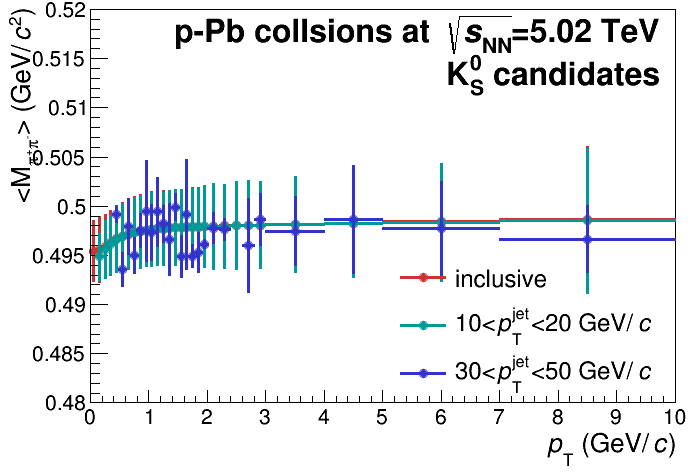
\includegraphics[width=.49\textwidth]{c04V0Reconstruction/KshortInvM}
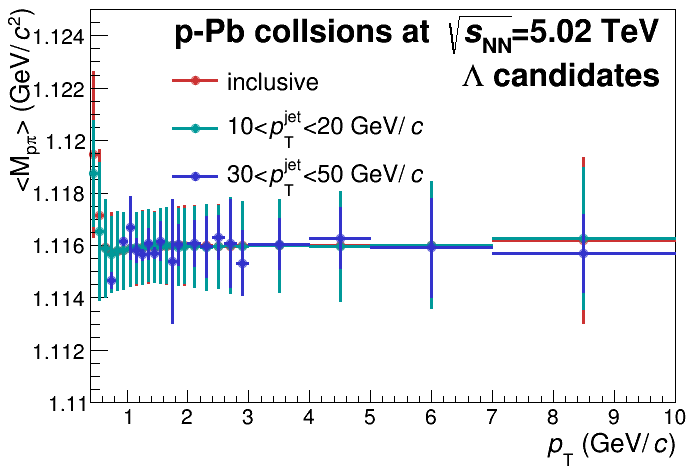
\includegraphics[width=.49\textwidth]{c04V0Reconstruction/LambdaInvM}
\caption{The mean and width of \Vzero\ invariant mass distribution extracted
         by the Gaussian fit for the inclusive $\Vzeros$ candidates
         and JC $\Vzero$ candidates as a function of $\pT$ in data.}
\label{fig:V0FitInvM}
\end{center}
\end{figure}

Figure~\ref{fig:V0FitInvM} shows the comparison of the mean and width of \Vzero\ invariant mass distribution extracted by the Gaussian fit for the inclusive \Vzeros\ candidates and JC \Vzero\ candidates as a function of $\pT$ in data.
The mean and width in the $\Vzero$ invariant mass distributions for the inclusive \Vzeros\ and JC \Vzeros\ are compatible within statistical uncertainties.
To avoid statistic fluctuations found in high-\pT\ jet selection, the number of JC \Vzeros is extracted using the mean and width obtained in the inclusive $\Vzero$ invariant mass distribution.

%%%%%%%%%%%%%%%%%%%%%%%%%%%%%%%%%%%%%%%%%%%%%%%%%%%%%%%%%%%%%%%%%%
\subsection{\Vzero\ particles from underlying event}
\label{sec:V0UE}

In order to measure the \Vzero\ yields in the underlying event (UE) (not associated to the hard scatterings tagged by the charged jets considered in this analysis) several estimators have been investigated:
\begin{itemize}
  \item the OC selection: the \Vzero\ particles that were not matched to any jet considered in the analysis within events containing a jet such that $\Delta R_{\Vzero-{\rm jet}} > R_{\rm cut}$;
  \item the PC selection: the \Vzero\ particles found in the perpendicular region (in the transverse plane) at angles larger than $\Delta \varphi = \varphi^{\rm jet} - \varphi^{\Vzero} > R_{\rm cut}$ \ask{(say the value)}
  \item the NJ selection: the \Vzero particles found in events that do not contain a jet with $\ptjet>5 \gevc$.
\end{itemize}

In practice, a useful quantity for performing the subtraction of the non-jet contribution of the \Vzero\ particles is their density per unit area $\rho^{\Vzero}(\pt)=N^{\Vzero}/A^{\Vzero}(\pt)$, where $A^{\Vzero}$ is the acceptance in pseudo-rapidity and azimuthal angle. Consequently, the number of the UE \Vzero\ particles within a jet can be calculated as $N=\rho^{\Vzero} \Ajet$ for each estimator separately. Note, in this analysis we consider the jet area \Ajet\ to be $\pi R^2$.

%%%%%%%%%%%%%%%%%%%%%%%%%%%%%%%%%%%%%%%%%%%%%%%%%%%%%%%%%%%%%%%%%%
\subsection{Efficiency}
\label{sec:c05V0EffiMC}

The efficiencies of \Vzero particles were estimated using DPMJET Monte Carlo generator \cite{Roesler:2000he} with the same cuts as in the data except the daughter track PID with ${\rm d}E/{\rm d}x$ in TPC. 
Figure~\ref{fig:c05EffiIncV0s} shows the efficiency of the inclusive $\Vzeros$ as a function of $\pT$ in three event multiplicity bins. For each of the event multiplicity class the efficiency is compared to the efficiency in minimum-bias events and it is found that the efficiency of inclusive $\Vzeros$ is independent on the event multiplicity.

\begin{figure}[htb]
\begin{center}
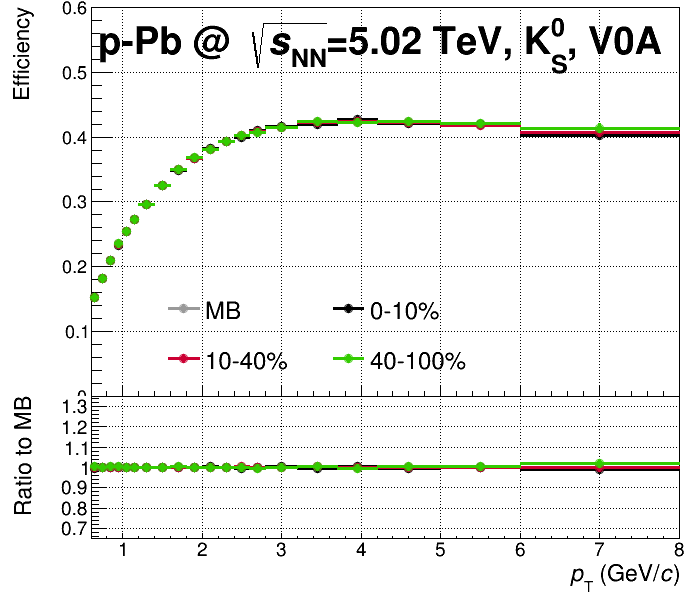
\includegraphics[width=.32\textwidth]{c04V0Reconstruction/cKshort_Efficiency}
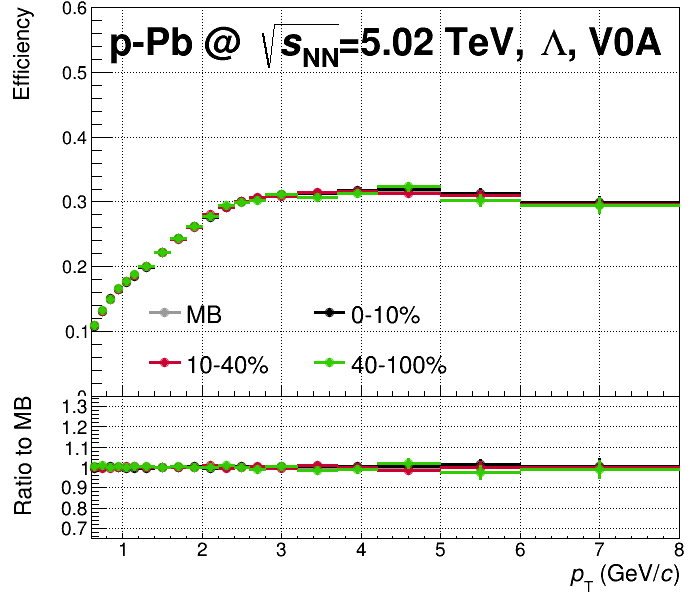
\includegraphics[width=.32\textwidth]{c04V0Reconstruction/cLambda_Efficiency}
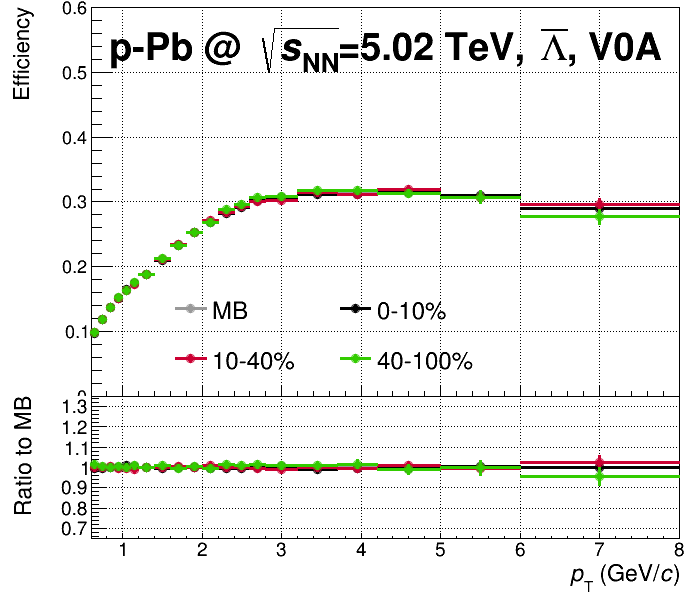
\includegraphics[width=.32\textwidth]{c04V0Reconstruction/cAntiLa_Efficiency}
\caption{Efficiency of inclusive $\Vzeros$ as a function of $\pT$ in three event multiplicity bins with V0A centrality estimator.}
\label{fig:c05EffiIncV0s}
\end{center}
\end{figure}

Due to differences in the experimental acceptance for \Vzero\ particles associated to jets (JC) and those extracted through the various estimators (OC, PC, NJ) of the underlying event the efficiencies of \Vzero\ particles were estimated separately in every case.

%%%%%%%%%%%%%%%%%%%%%%%%%%%%%%%%%%%%%%%%%%%%%%%%%%%%%%%%%%%%%%%%%%
\subsection{Feed-down subtraction for \lda\ and \alda}

The \pt\ differential yields of \lda\ and \alda\ reconstructed for each selection (JC and UE selections) where corrected for the feed-down from $\Xi$ decays. 
%%The correction was applied before the efficiency corrections. 
The $\Xi$ production in jets (JC) was estimated based on measurements of the multi-strange baryons and their decays at high-\pt\ performed in \pp\ collisions \cite{Abelev:2012jp} and extrapolated to the lower \pt\ using PYTHIA event generator and full detector simulations.

%!TEX root = ../AliPubV0JetspPb.tex

\section{Results}

The final results with different jet $\pT$ thresholds and event
multiplicity estimators are listed in this section:
\begin{itemize}
\item figure~\ref{fig:c07PtJ10V0A}:
      results in $\pT^{\rm jet}>10~\GeVc$
      with V0A event multiplicity estimator;
\item figure~\ref{fig:c07PtJ20V0A}:
      results in $\pT^{\rm jet}>20~\GeVc$
      with V0A event multiplicity estimator;
\item figure~\ref{fig:c07PtJ10ZNA}:
      results in $\pT^{\rm jet}>10~\GeVc$
      with ZNA event multiplicity estimator;
\item figure~\ref{fig:c07PtJ20ZNA}:
      results in $\pT^{\rm jet}>20~\GeVc$
      with ZNA event multiplicity estimator.
\end{itemize}

\begin{figure}[htb]
\begin{center}
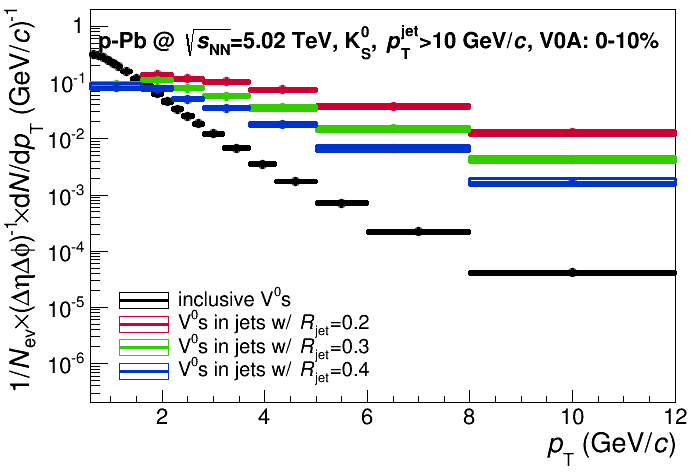
\includegraphics[width=.32\textwidth]{c07PtJ10V0A/cKshort_0.png}
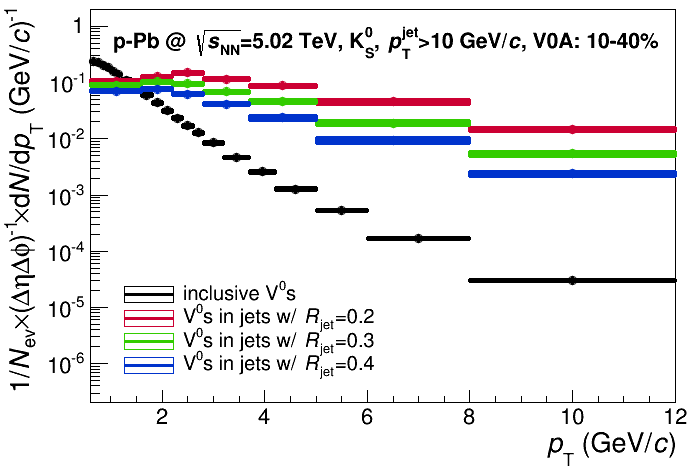
\includegraphics[width=.32\textwidth]{c07PtJ10V0A/cKshort_1.png}
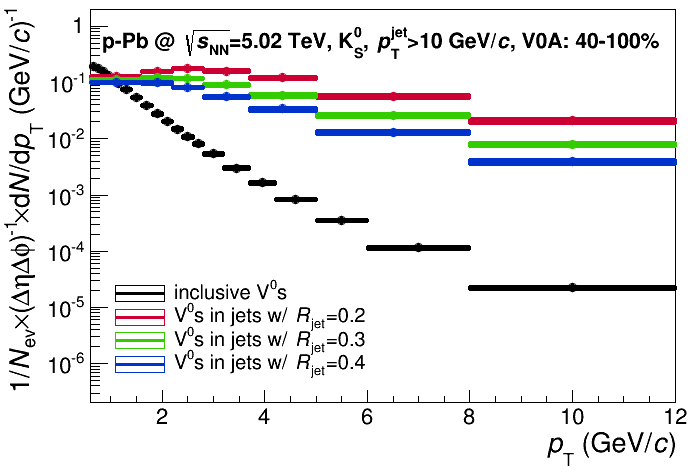
\includegraphics[width=.32\textwidth]{c07PtJ10V0A/cKshort_2.png}
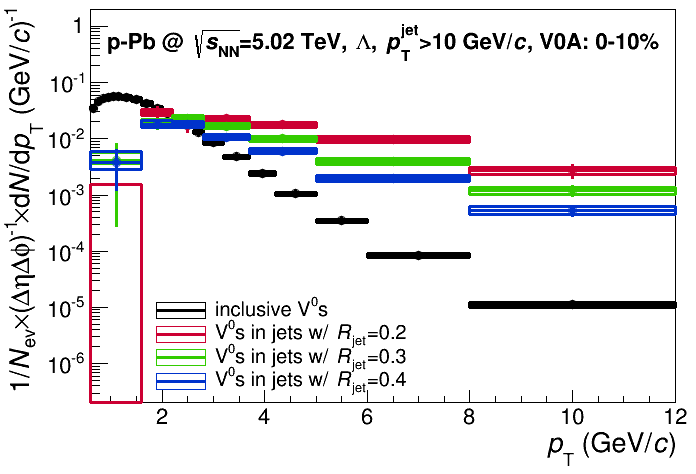
\includegraphics[width=.32\textwidth]{c07PtJ10V0A/cLambda_0.png}
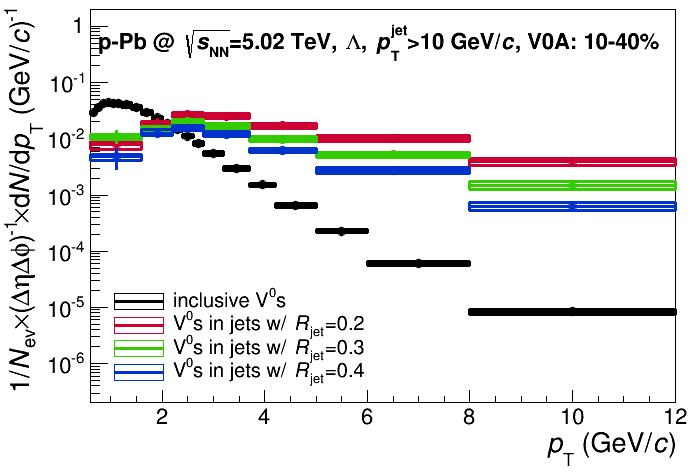
\includegraphics[width=.32\textwidth]{c07PtJ10V0A/cLambda_1.png}
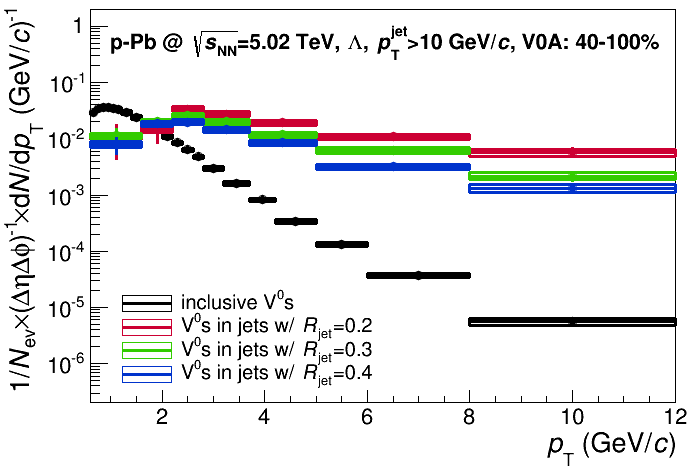
\includegraphics[width=.32\textwidth]{c07PtJ10V0A/cLambda_2.png}
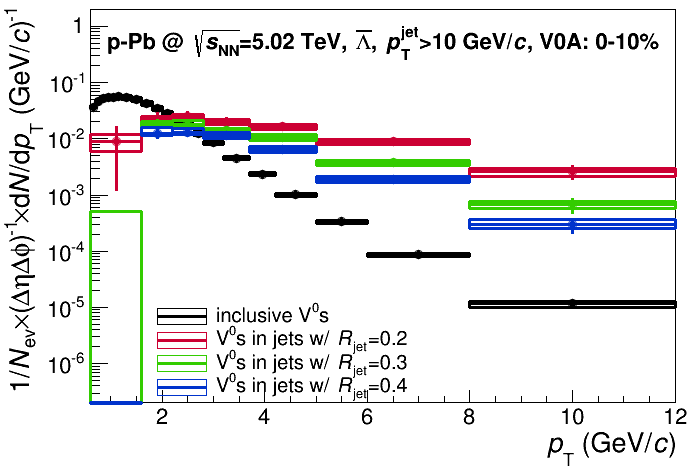
\includegraphics[width=.32\textwidth]{c07PtJ10V0A/cAntiLa_0.png}
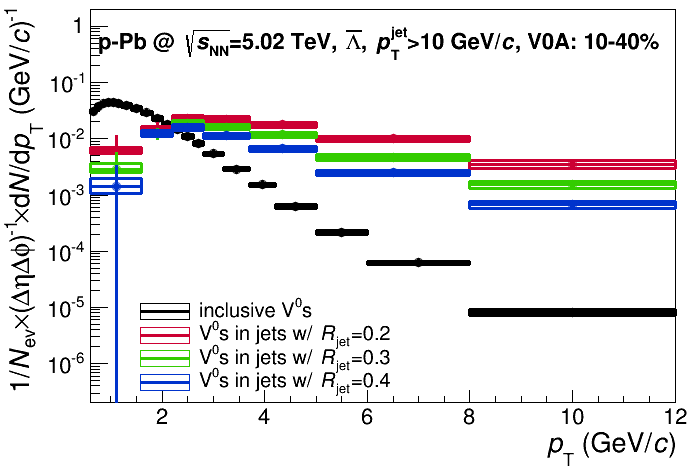
\includegraphics[width=.32\textwidth]{c07PtJ10V0A/cAntiLa_1.png}
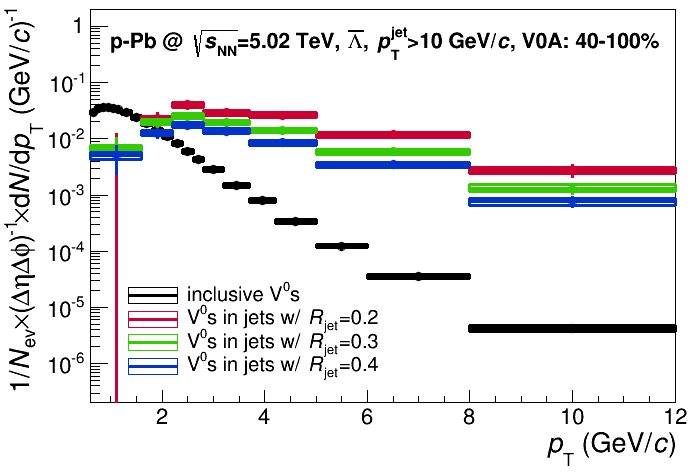
\includegraphics[width=.32\textwidth]{c07PtJ10V0A/cAntiLa_2.png}
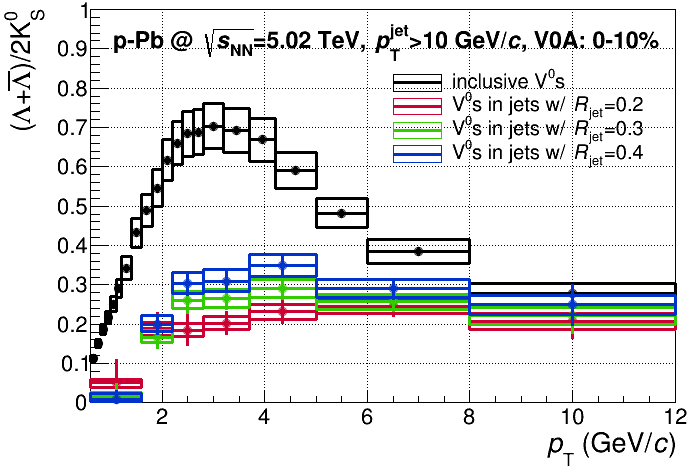
\includegraphics[width=.32\textwidth]{c07PtJ10V0A/cRatioV_0.png}
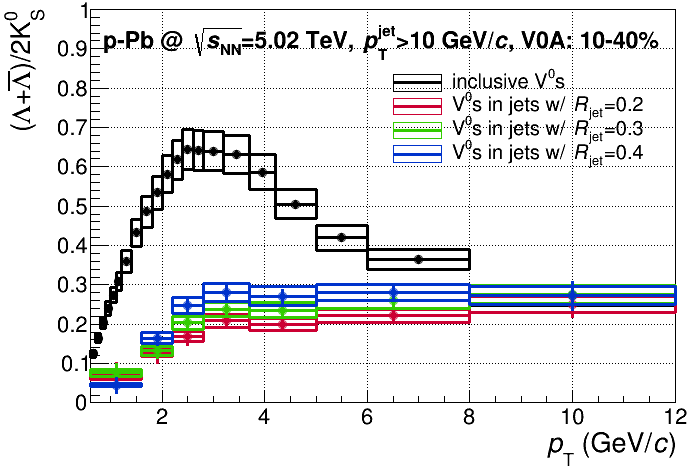
\includegraphics[width=.32\textwidth]{c07PtJ10V0A/cRatioV_1.png}
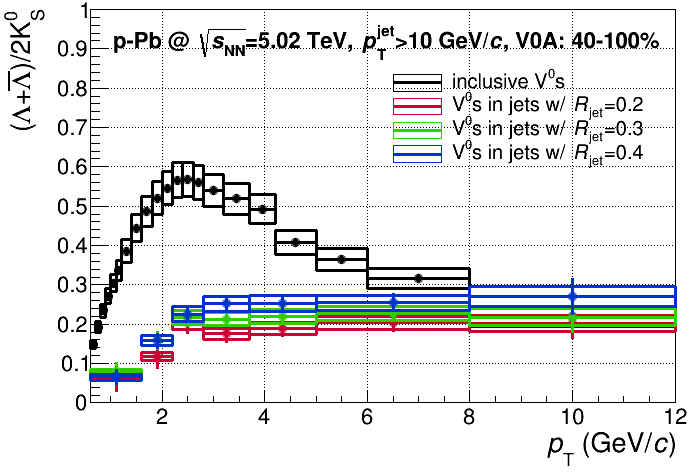
\includegraphics[width=.32\textwidth]{c07PtJ10V0A/cRatioV_2.png}
\caption{Results in jet $\pT>10~\GeVc$ with V0A centrality estimator.}
\label{fig:c07PtJ10V0A}
\end{center}
\end{figure}
 
\begin{figure}[htb]
\begin{center}
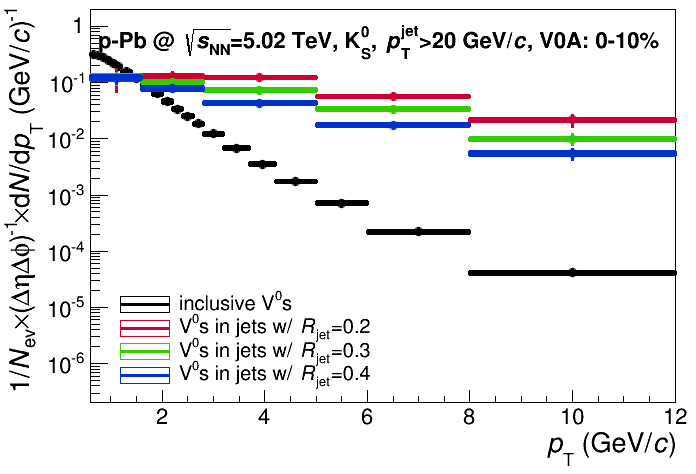
\includegraphics[width=.32\textwidth]{c07PtJ20V0A/cKshort_0.png}
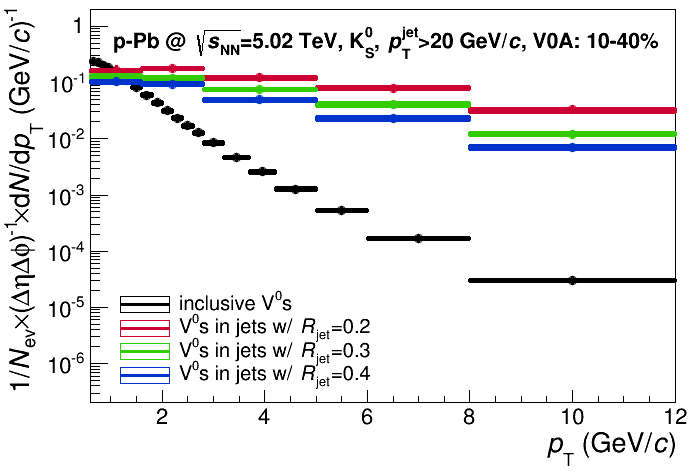
\includegraphics[width=.32\textwidth]{c07PtJ20V0A/cKshort_1.png}
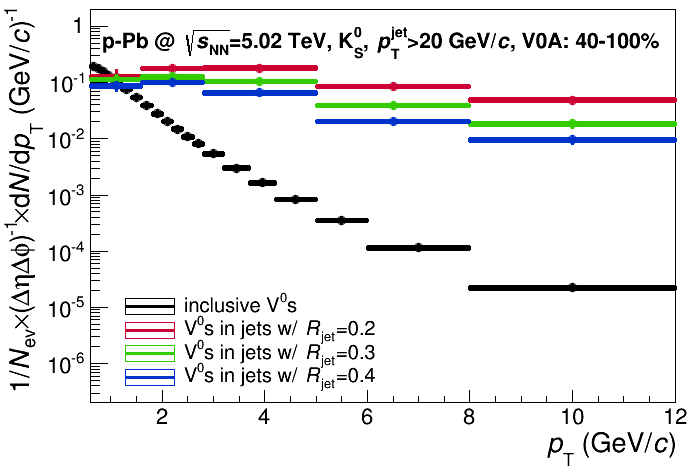
\includegraphics[width=.32\textwidth]{c07PtJ20V0A/cKshort_2.png}
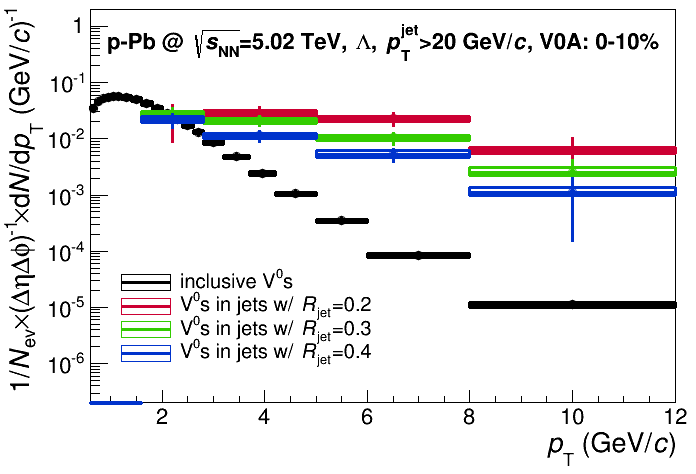
\includegraphics[width=.32\textwidth]{c07PtJ20V0A/cLambda_0.png}
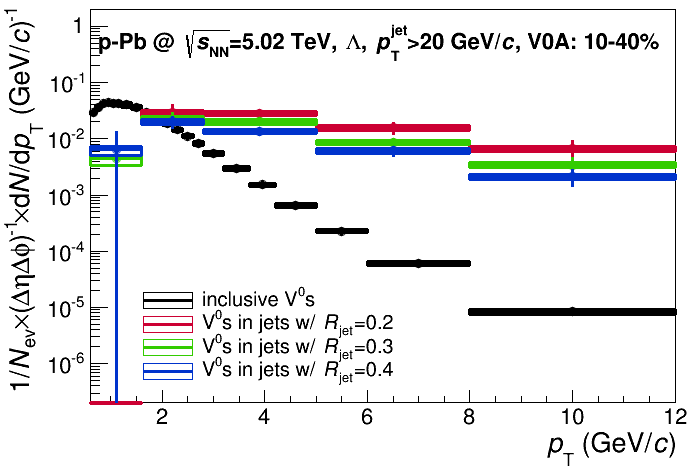
\includegraphics[width=.32\textwidth]{c07PtJ20V0A/cLambda_1.png}
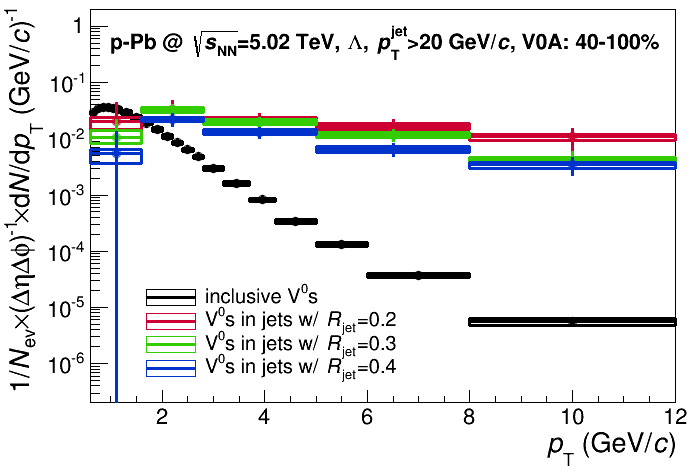
\includegraphics[width=.32\textwidth]{c07PtJ20V0A/cLambda_2.png}
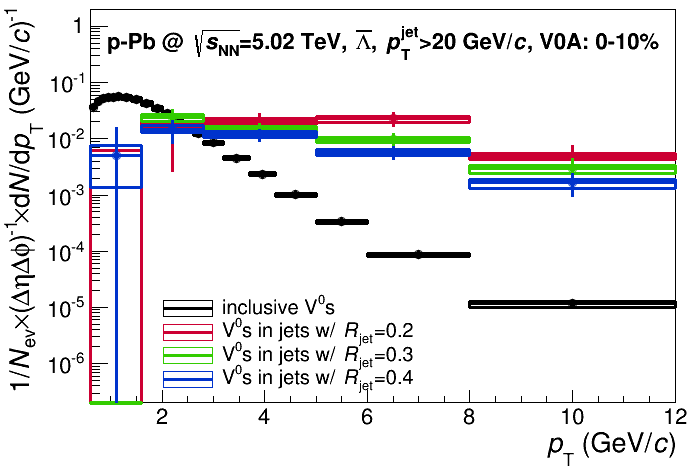
\includegraphics[width=.32\textwidth]{c07PtJ20V0A/cAntiLa_0.png}
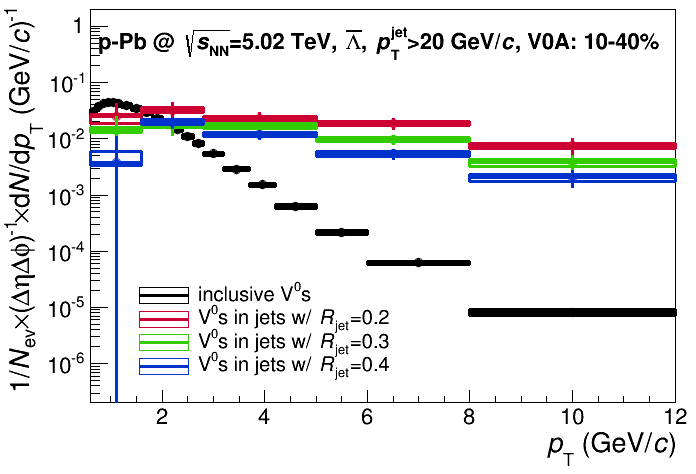
\includegraphics[width=.32\textwidth]{c07PtJ20V0A/cAntiLa_1.png}
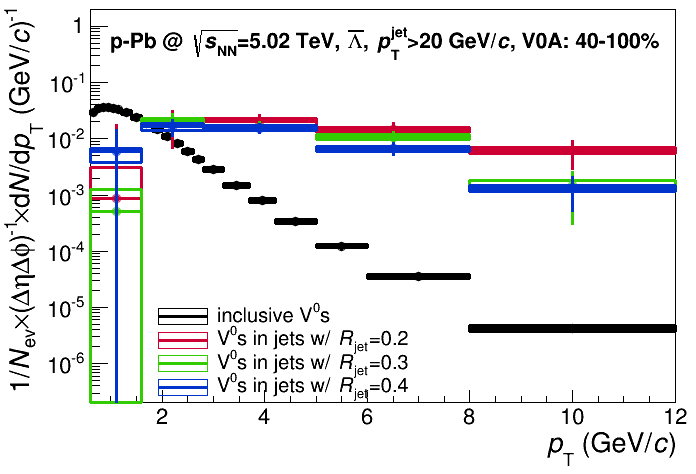
\includegraphics[width=.32\textwidth]{c07PtJ20V0A/cAntiLa_2.png}
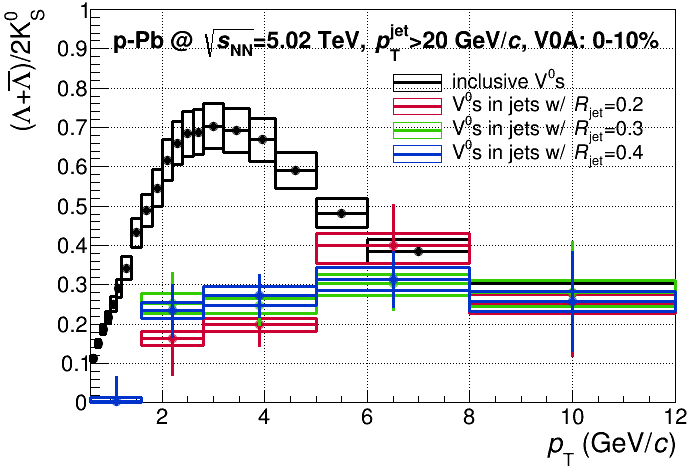
\includegraphics[width=.32\textwidth]{c07PtJ20V0A/cRatioV_0.png}
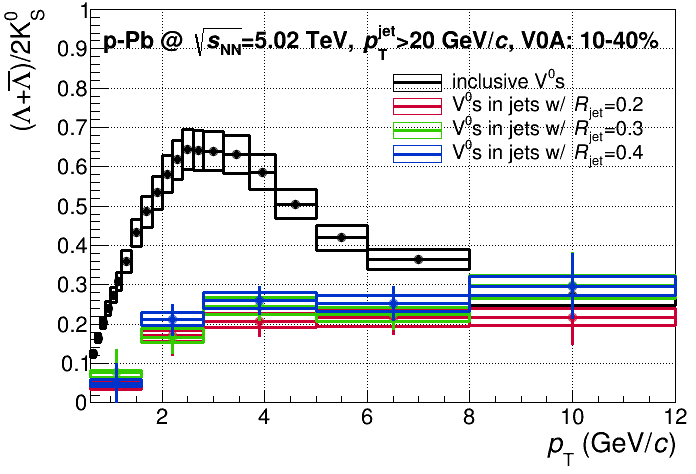
\includegraphics[width=.32\textwidth]{c07PtJ20V0A/cRatioV_1.png}
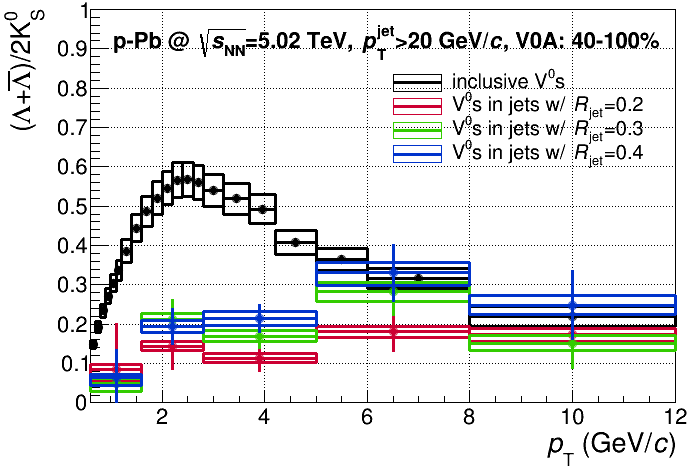
\includegraphics[width=.32\textwidth]{c07PtJ20V0A/cRatioV_2.png}
\caption{Results in jet $\pT>20~\GeVc$ with V0A centrality estimator.}
\label{fig:c07PtJ20V0A}
\end{center}
\end{figure}
 
\begin{figure}[htb]
\begin{center}
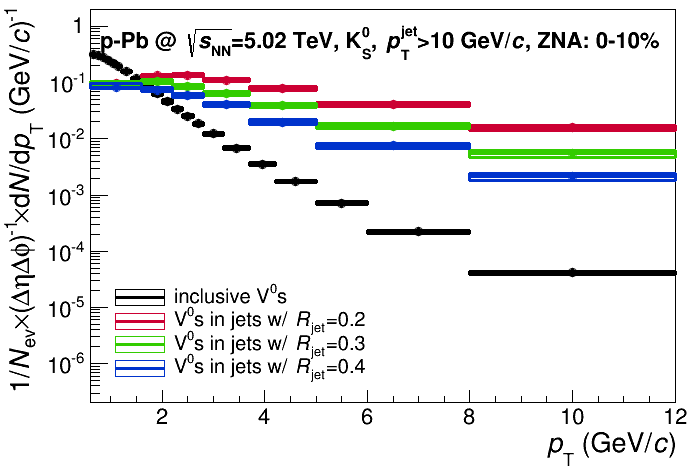
\includegraphics[width=.32\textwidth]{c07PtJ10ZNA/cKshort_0.png}
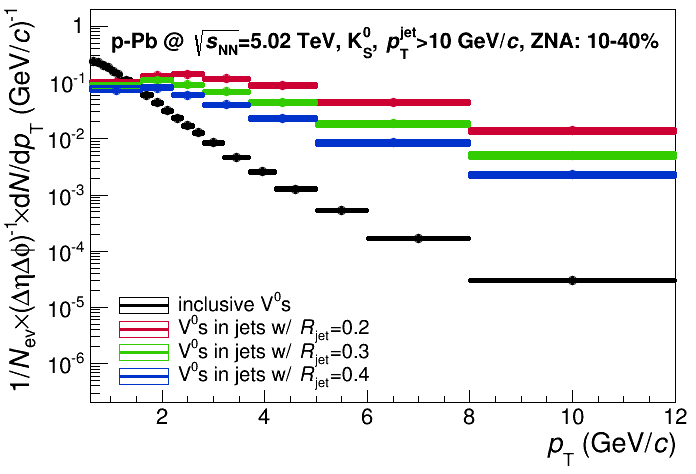
\includegraphics[width=.32\textwidth]{c07PtJ10ZNA/cKshort_1.png}
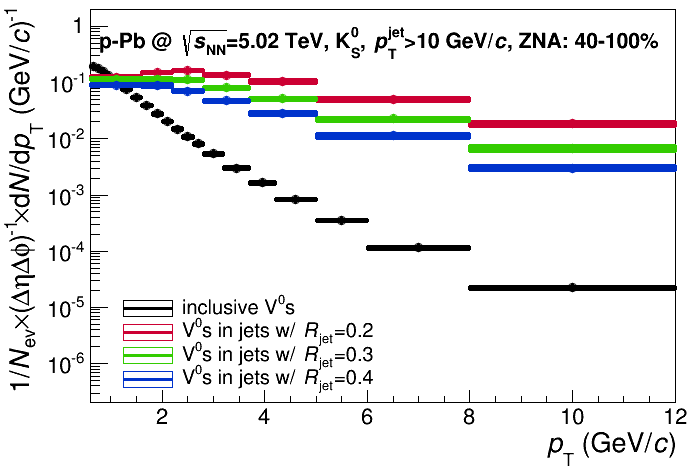
\includegraphics[width=.32\textwidth]{c07PtJ10ZNA/cKshort_2.png}
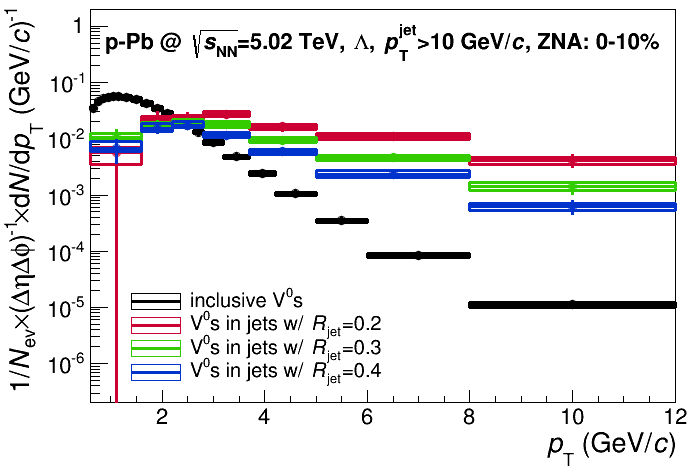
\includegraphics[width=.32\textwidth]{c07PtJ10ZNA/cLambda_0.png}
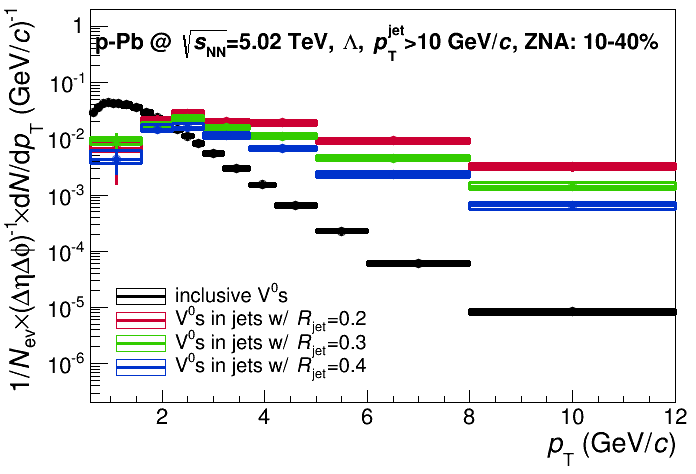
\includegraphics[width=.32\textwidth]{c07PtJ10ZNA/cLambda_1.png}
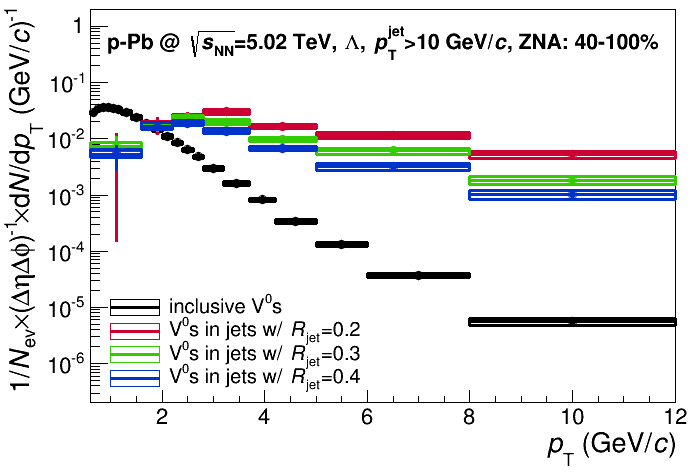
\includegraphics[width=.32\textwidth]{c07PtJ10ZNA/cLambda_2.png}
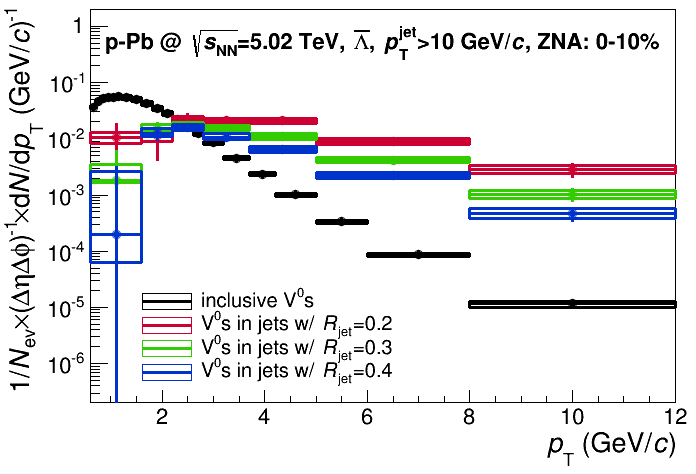
\includegraphics[width=.32\textwidth]{c07PtJ10ZNA/cAntiLa_0.png}
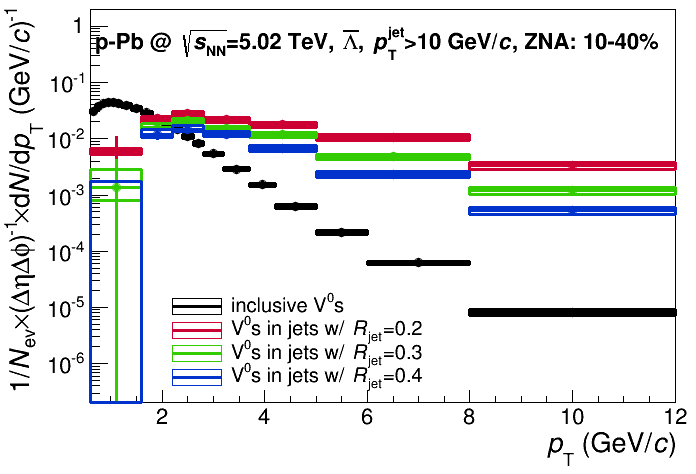
\includegraphics[width=.32\textwidth]{c07PtJ10ZNA/cAntiLa_1.png}
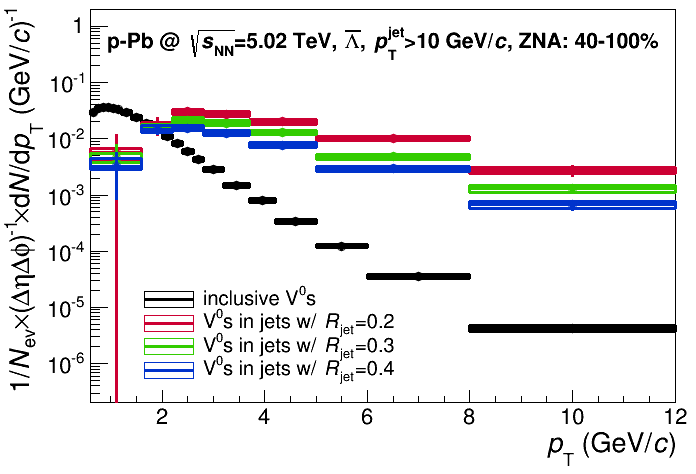
\includegraphics[width=.32\textwidth]{c07PtJ10ZNA/cAntiLa_2.png}
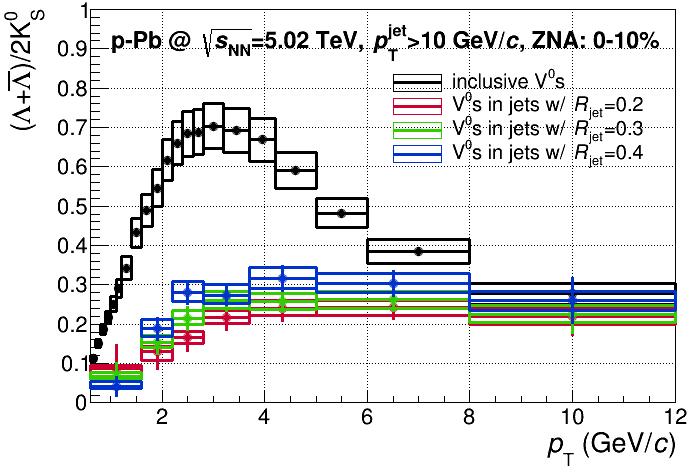
\includegraphics[width=.32\textwidth]{c07PtJ10ZNA/cRatioV_0.png}
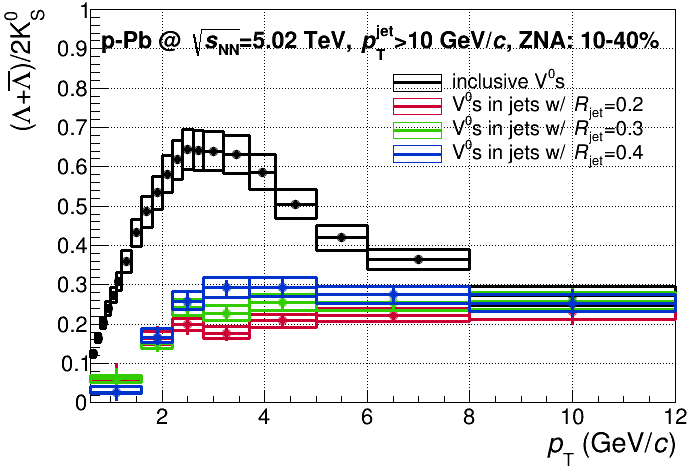
\includegraphics[width=.32\textwidth]{c07PtJ10ZNA/cRatioV_1.png}
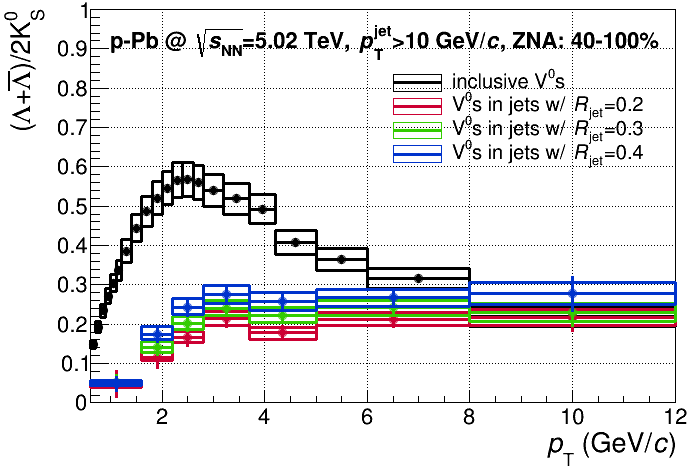
\includegraphics[width=.32\textwidth]{c07PtJ10ZNA/cRatioV_2.png}
\caption{Results in jet $\pT>10~\GeVc$ with ZNA centrality estimator.}
\label{fig:c07PtJ10ZNA}
\end{center}
\end{figure}
 
\begin{figure}[htb]
\begin{center}
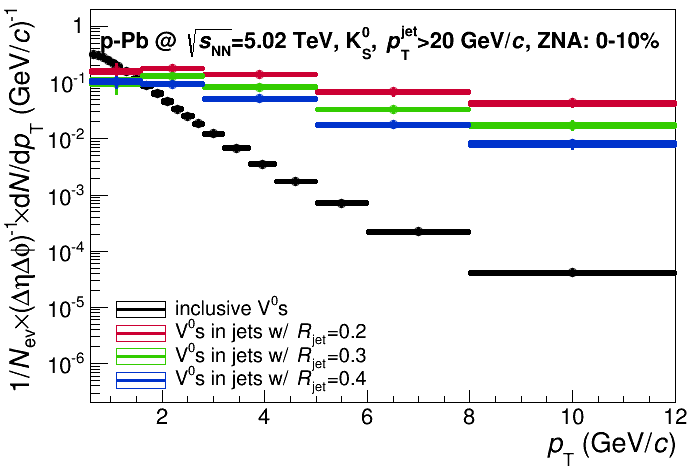
\includegraphics[width=.32\textwidth]{c07PtJ20ZNA/cKshort_0.png}
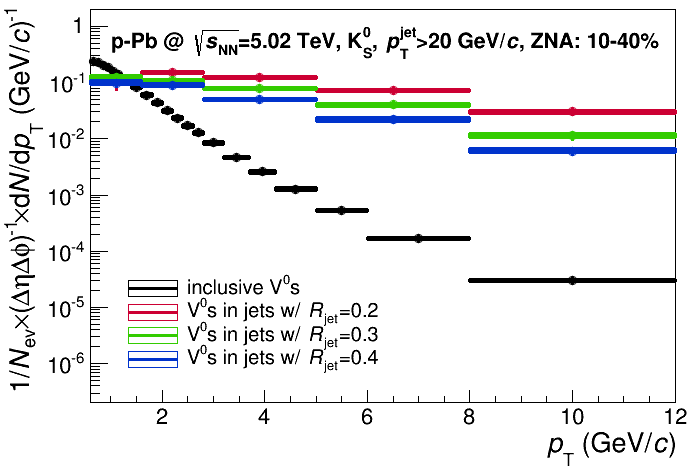
\includegraphics[width=.32\textwidth]{c07PtJ20ZNA/cKshort_1.png}
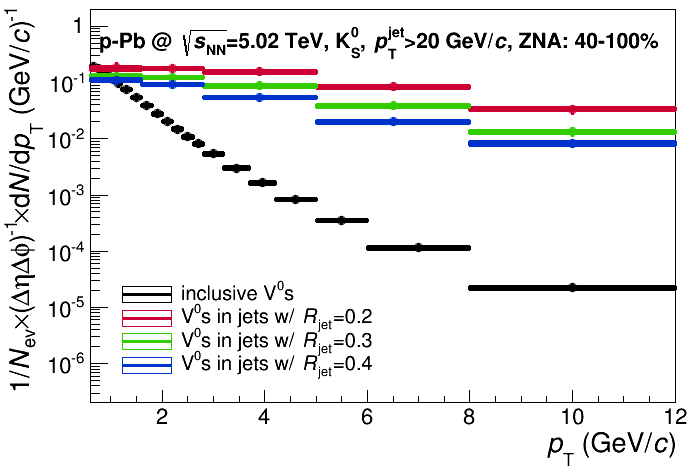
\includegraphics[width=.32\textwidth]{c07PtJ20ZNA/cKshort_2.png}
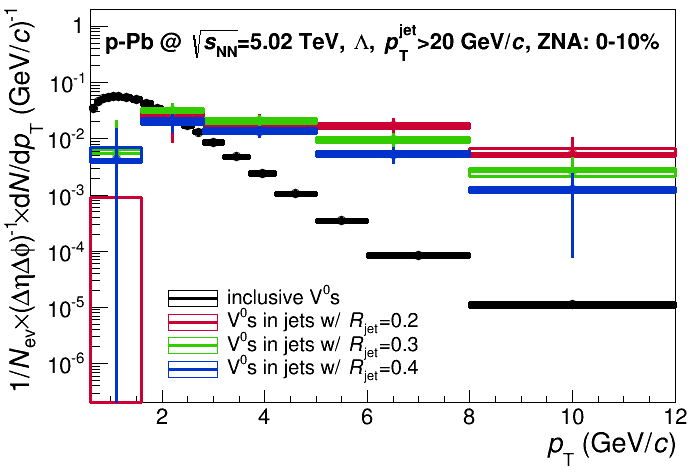
\includegraphics[width=.32\textwidth]{c07PtJ20ZNA/cLambda_0.png}
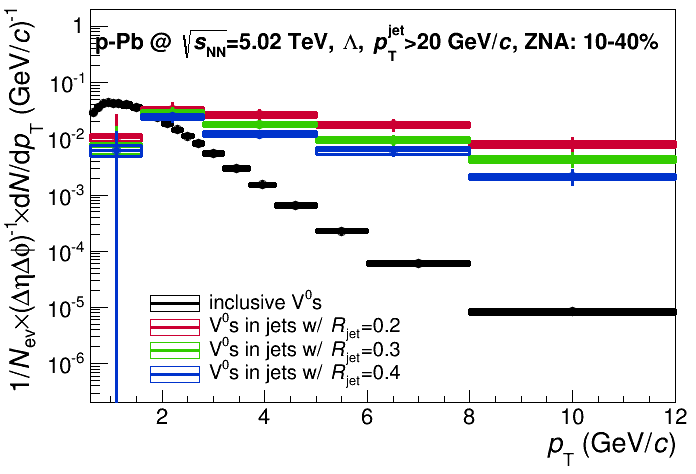
\includegraphics[width=.32\textwidth]{c07PtJ20ZNA/cLambda_1.png}
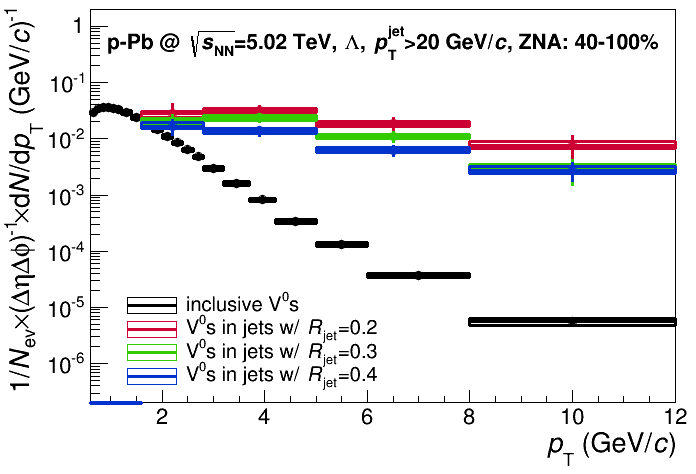
\includegraphics[width=.32\textwidth]{c07PtJ20ZNA/cLambda_2.png}
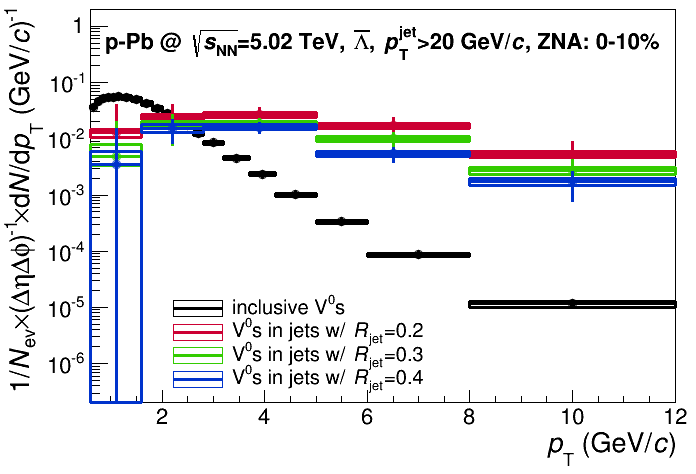
\includegraphics[width=.32\textwidth]{c07PtJ20ZNA/cAntiLa_0.png}
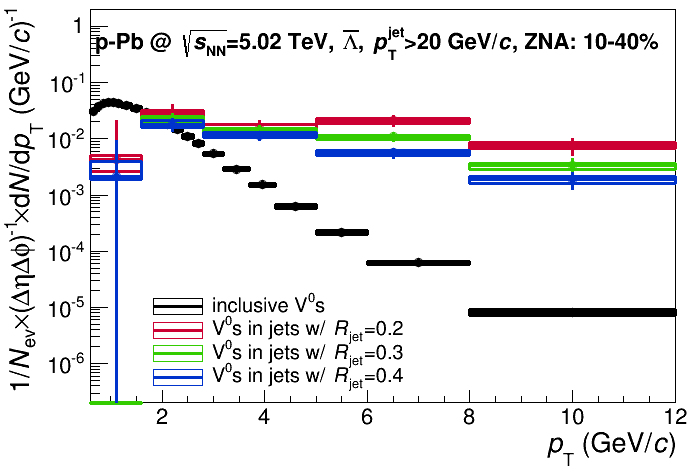
\includegraphics[width=.32\textwidth]{c07PtJ20ZNA/cAntiLa_1.png}
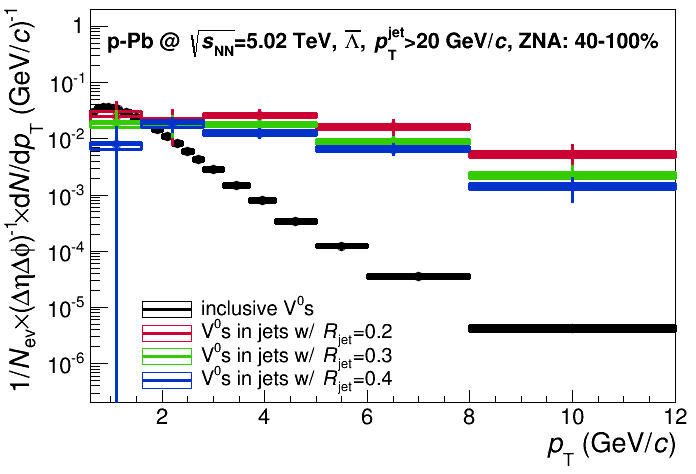
\includegraphics[width=.32\textwidth]{c07PtJ20ZNA/cAntiLa_2.png}
\includegraphics[width=.32\textwidth]{c07PtJ20ZNA/cRatioV_0.png}
\includegraphics[width=.32\textwidth]{c07PtJ20ZNA/cRatioV_1.png}
\includegraphics[width=.32\textwidth]{c07PtJ20ZNA/cRatioV_2.png}
\caption{Results in jet $\pT>20~\GeVc$ with ZNA centrality estimator.}
\label{fig:c07PtJ20ZNA}
\end{center}
\end{figure}

%!TEX root = ../AliPubV0JetspPb.tex

\section{Systematic uncertainties}
\label{sec:uncertainties}

\ask{sections below need more quant. and phrasing to be checked; also add a summary figure as a function \pt}

The systematic uncertainties on the particle spectra and their ratios originating from the sources discussed below are added in quadrature.

\subsection{Uncertainties in \Vzero\ particle reconstruction}

The dominant sources of the systematic uncertainties for the \Vzero particle reconstruction are summarized in Table \ref{tab:v0syst}.

\begin{table}[t]
\centering 
\begin{tabular*}{\linewidth}{@{\extracolsep{\fill}}lccc}
\hline
&&&\\[-0.7em]
 & \kzero\ & \multicolumn{2}{c}{\lmb(\almb)}\\[0.3em]
\hline
&&&\\[-0.7em]
Proper lifetime & 2\% & \multicolumn{2}{c}{2\%} \\[0.3em]
Material budget & 4\% & \multicolumn{2}{c}{4\%} \\[0.3em]
Track selection  & 4\% & \multicolumn{2}{c}{4\%} \\[0.3em]
TPC PID & 1\% & \multicolumn{2}{c}{1\%} \\[0.3em]
Multiplicity & \multirow{2}{*}{2\%} & \multicolumn{2}{c}{\multirow{2}{*}{2\%}} \\
dependence & & \\[0.3em]
\hline
\hline
&&&\\[-0.7em]
\pt\ (\gevc)  &  & $<$ 3.7 & $>$ 3.7\\[0.3em]
\hline
&&&\\[-0.7em]
Feed-down  &  & \multirow{2}{*}{5\%} & \multirow{2}{*}{7\%}\\
correction & & &\\[0.3em]
    \hline
    \hline
    &&&\\[-0.7em]
\pt\ (\gevc)  &  & $<$ 3.7 & $>$ 3.7\\[0.3em]
    \hline
    &&&\\[-0.7em]
    Total & 6.5\% & 8\% & 9.5\% \\[0.3em]
\hline
\end{tabular*}
\caption{Main sources of systematic uncertainty for the \kzero\ and \lmb(\almb).} \label{tab:v0syst}
\end{table}

\subsection{Uncertainty in UE \Vzero\ estimation}

The uncertainties originating from the mis-association of \Vzero particles with UE were considered. The two main sources arise from cases where:
\begin{itemize}
\item the \Vzero\ particle was found outside the selected jet and classified as UE particle; however, it may have originated by a physical jet outside the fiducial acceptance for jets considered in the analysis and/or originates from a true low-\pt jet, below the considered thresholds;
\item the \Vzero\ particle originates from true high-\pt jet; however, due to the finite detector efficiency the jet has not been reconstructed above the considered \pt\ thresholds.
\end{itemize}
The uncertainty on the UE \Vzero density has been estimated using the two variations of the UE estimators: the OC and the NJ. The difference in the reconstructed \Vzero\ yields with the different estimators has been included as the additional systematic uncertainties on the yield of particles within the jets.

\subsection{Jet reconstruction and jet selection}

The systematic uncertainty originating from the selection of the jet \pt\ were estimated by repeating the analysis with jet \pt\ varied around the chosen 10 and 20 \gevc\ thresholds by 2 \gevc. This variation accounts for jet resolution due to detector effects and the fluctuations of the event background density as reported in \cite{Adam:2015hoa}. \ask{numbers needed}. 


%!TEX root = ../AliPubV0JetspPb.tex

\section{Summary}

\begin{enumerate}
	\item spectra harder in jets
	\item L/K ratio: a) different than inclusive or OC/PC/NJ/inclusive - no peak; b) consistent with vacuum within uncertainties -> UE radial flow; jets do not flow
	\item mean \pt -> hint softening of jet fragments in most central collisions? - tension with 2.b
	\item constraint on the soft-hard parton recombination (?)
\end{enumerate}


%==========================================================%
%======================ACK+BIBLIO==========================%
%==========================================================%
\ifpreprint
\iffull
\newenvironment{acknowledgement}{\relax}{\relax}
\begin{acknowledgement}
\section*{Acknowledgements}
The ALICE Collaboration would like to thank all its engineers and technicians
for their invaluable contributions to the construction of the experiment and
the CERN accelerator teams for the outstanding performance of the LHC complex.
%
The ALICE Collaboration gratefully acknowledges the resources and support
provided by all Grid centres and the Worldwide LHC Computing Grid (WLCG)
collaboration.
%
The ALICE Collaboration acknowledges the following funding agencies for
their support in building and running the ALICE detector:
%
State Committee of Science,  World Federation of Scientists (WFS)
and Swiss Fonds Kidagan, Armenia,
%
Conselho Nacional de Desenvolvimento Cient\'{\i}fico e Tecnol\'{o}gico (CNPq),
Financiadora de Estudos e Projetos (FINEP),
Funda\c{c}\~{a}o de Amparo \`{a} Pesquisa do Estado de S\~{a}o Paulo (FAPESP);
%
National Natural Science Foundation of China (NSFC),
the Chinese Ministry of Education (CMOE)
and the Ministry of Science and Technology of China (MSTC);
%
Ministry of Education and Youth of the Czech Republic;
%
Danish Natural Science Research Council,
the Carlsberg Foundation and the Danish National Research Foundation;
%
The European Research Council under the European Community's
Seventh Framework Programme;
%
Helsinki Institute of Physics and the Academy of Finland;
%
French CNRS-IN2P3,
the `Region Pays de Loire', `Region Alsace', `Region Auvergne' and CEA, France;
%
German Bundesministerium fur Bildung, Wissenschaft,
Forschung und Technologie (BMBF) and the Helmholtz Association;
%
General Secretariat for Research and Technology, Ministry of
Development, Greece;
%
Hungarian Orszagos Tudomanyos Kutatasi Alappgrammok (OTKA) and
National Office for Research and Technology (NKTH);
%
Department of Atomic Energy and Department of Science and Technology of the
Government of India;
%
Istituto Nazionale di Fisica Nucleare (INFN) and Centro Fermi -
Museo Storico della Fisica e Centro Studi e Ricerche "Enrico Fermi", Italy;
%
MEXT Grant-in-Aid for Specially Promoted Research, Ja\-pan;
%
Joint Institute for Nuclear Research, Dubna;
%
National Research Foundation of Korea (NRF);
%
Consejo Nacional de Cienca y Tecnologia (CONACYT),
Direccion General de Asuntos del Personal Academico(DGAPA),
M\'{e}xico, :Amerique Latine Formation academique –
European Commission(ALFA-EC) and the EPLANET Program (European
Particle Physics Latin American Network)
%
Stichting voor Fundamenteel Onderzoek der Materie (FOM) and
the Nederlandse Organisatie voor Wetenschappelijk Onderzoek (NWO), Netherlands;
%
Research Council of Norway (NFR);
%
Polish Ministry of Science and Higher Education;
%
National Science Centre, Poland;
%
Ministry of National Education/Institute for Atomic Physics and
Consiliul Naţional al Cercetării Ştiinţifice -
Executive Agency for Higher Education Research Development and
Innovation Funding (CNCS-UEFISCDI) - Romania;
%
Ministry of Education and Science of Russian Federation, Russian
Academy of Sciences, Russian Federal Agency of Atomic Energy,
Russian Federal Agency for Science and Innovations and The Russian
Foundation for Basic Research;
%
Ministry of Education of Slovakia;
%
Department of Science and Technology, South Africa;
%
Centro de Investigaciones Energeticas,
Medioambientales y Tecnologicas (CIEMAT),
E-Infrastructure shared between Europe and Latin America (EELA),
Ministerio de Econom\'{i}a y Competitividad (MINECO) of Spain,
Xunta de Galicia (Conseller\'{\i}a de Educaci\'{o}n),
Centro de Aplicaciones Tecnológicas y Desarrollo Nuclear (CEA\-DEN),
Cubaenerg\'{\i}a, Cuba, and IAEA (International Atomic Energy Agency);
%
Swedish Research Council (VR) and Knut $\&$ Alice Wallenberg
Foundation (KAW);
%
Ukraine Ministry of Education and Science;
%
United Kingdom Science and Technology Facilities Council (STFC);
%
The United States Department of Energy, the United States National
Science Foundation, the State of Texas, and the State of Ohio;
%
Ministry of Science, Education and
Sports of Croatia and  Unity through Knowledge Fund, Croatia.
%
Council of Scientific and Industrial Research (CSIR), New Delhi, India
        %%%%%%% get the latest version before submitting
\end{acknowledgement}
\ifbibtex
\bibliographystyle{\bibstname}
\bibliography{AliPubV0JetspPb}{}
\else
\input{refpreprint.tex}
\fi
\newpage
\appendix
\section{The ALICE Collaboration}
\label{app:collab}
\input{authors-preprint.tex}        %%%%%%% get the latest version before submitting
\else
\ifbibtex
\bibliographystyle{\bibstname}
\bibliography{AliPubV0JetspPb}
\else
\ifpreprint
  \documentclass[ALICE,manyauthors,12pt]{cernphprep}
  \usepackage[comma,square,numbers,sort&compress]{natbib}
  \usepackage{booktabs}
\else %%% PUT PAPER STYLE BELOW %%%
  \ifplbpaper
  \documentclass[final,3p,12pt]{elsarticle}
  \biboptions{comma,square,numbers,sort&compress}
  \def\bibstname{utphys}
  \fi
%
  \ifapspaper
  \documentclass[10pt,aps,prl,superscriptaddress,altaffilletter,nobibnotes,nofootinbib]{revtex4-1}
  \newenvironment{frontmatter}{}{\maketitle}
  \def\bibstname{apsrev4-1}
  \fi
\fi
%%%%%%%%%%%%%%%%%%%%%%%%%%%%%%%%%%%%%%%%%%%%%%%%%%%%%%%%%%%%%%%%%%%%%%%%%%%%%%%

\ifdraft
  \usepackage{lineno}
  \linenumbers
  \setlength\linenumbersep{0.06in}
  \modulolinenumbers[5]
  \usepackage{fancyhdr}
  \pagestyle{fancyplain}
  \fancyhead{}
  \fancyhead[L,L]{\color{red}ALICE INTERNAL ONLY}
  \fancyhead[R,R]{\thepage}
  \fancyfoot{}
  \fancyfoot[L,L]{\color{red}DRAFT \dvers\ \revision $\color{white}:$\$}
  \fancyfoot[R,R]{\color{red} \today $\color{white}:$\$}
  \renewcommand{\headrulewidth}{0pt} % remove lines as well
  \renewcommand{\footrulewidth}{0pt}
  \newcommand{\ask}[1]{\textcolor{magenta}{#1}}
\else
  \newcommand{\ask}[1]{}
\fi
%%%%%%%%%%%%%%%%%%%%%%%%%%%%%%%%%%%%%%%%%%%%%%%%%%%%%%%%%%%%%%%%%%%%%%%%%%%%%%%

\iflatexdiff
  \RequirePackage{color}
  \definecolor{RED}{rgb}{1,0,0}
  \definecolor{BLUE}{rgb}{0,0,1}
  \providecommand{\DIFadd}[1]{{\protect\color{blue}\uwave{#1}}}
  \providecommand{\DIFdel}[1]{{\protect\color{red}\sout{#1}}}
  \providecommand{\DIFaddbegin}{}
  \providecommand{\DIFaddend}{}
  \providecommand{\DIFdelbegin}{}
  \providecommand{\DIFdelend}{}
  \providecommand{\DIFaddFL}[1]{\DIFadd{#1}}
  \providecommand{\DIFdelFL}[1]{\DIFdel{#1}}
  \providecommand{\DIFaddbeginFL}{}
  \providecommand{\DIFaddendFL}{}
  \providecommand{\DIFdelbeginFL}{}
  \providecommand{\DIFdelendFL}{}
\fi
%==========================================================%

\usepackage{float}
\usepackage{rotating}

\usepackage{graphicx}
\usepackage{graphics}
\usepackage{epstopdf}
\usepackage{epsfig}
\usepackage{grffile}

\usepackage{dcolumn}
\usepackage{multirow}
\usepackage{array}

\usepackage{bm}
\usepackage{amsmath}
\usepackage{amssymb}
\usepackage{amsfonts}

\usepackage{units}
\usepackage{hyperref}

\usepackage{color}
%\usepackage[usenames]{color}

\usepackage{textcomp}
\usepackage[normalem]{ulem}
\usepackage[utf8]{inputenc}
\usepackage[T1]{fontenc}

%usepackage{changes}
%usepackage{lipsum}
%definechangesauthor[name={Xiaoming Zhang}, color=orange]{xz}
%definechangesauthor[name={MP}, color=orange]{mp}
%setremarkmarkup{(#2)}
%%%%%%%%%%%%%%%%%%%%%%%%%%%%%%%%%%%%%%%%%%%%%%%%%%%%%%%%%%%%%%%%%%%%%%%%%%%%%%%

\graphicspath{{figures/}
              {figures/c00Logos/}
              {figures/c23V0Reco/}
              {figures/c24Syst/}
              {figures/c03Results/}}
%%%%%%%%%%%%%%%%%%%%%%%%%%%%%%%%%%%%%%%%%%%%%%%%%%%%%%%%%%%%%%%%%%%%%%%%%%%%%%%

\newcolumntype{P}[1]{>{\centering\arraybackslash}p{#1}}
\newcolumntype{M}[1]{>{\centering\arraybackslash}m{#1}}
%%%%%%%%%%%%%%%%%%%%%%%%%%%%%%%%%%%%%%%%%%%%%%%%%%%%%%%%%%%%%%%%%%%%%%%%%%%%%%%

\newcommand{\murm}{%
  \ifmmode
    \mathchoice
        {\hbox{\normalsize\textmu}}
        {\hbox{\normalsize\textmu}}
        {\hbox{\scriptsize\textmu}}
        {\hbox{\tiny\textmu}}%
  \else
    \textmu
  \fi
}
%%%%%%%%%%%%%%%%%%%%%%%%%%%%%%%%%%%%%%%%%%%%%%%%%%%%%%%%%%%%%%%%%%%%%%%%%%%%%%%

\newcommand{\pip}{\ensuremath{\pi^{+}}}
\newcommand{\pim}{\ensuremath{\pi^{-}}}
\newcommand{\kap}{\ensuremath{{\rm K}^{+}}}
\newcommand{\kam}{\ensuremath{{\rm K}^{-}}}
\newcommand{\pbar}{\ensuremath{\rm\overline{p}}}
\newcommand{\degree}{\ensuremath{^{\rm o}}}
\newcommand{\s}{\ensuremath{\sqrt{s}}}
\newcommand{\pt}{\ensuremath{p_{\rm t}}}
\newcommand{\dedx}{\ensuremath{{\rm d}E/{\rm d}x}}
\newcommand{\dndy}{\ensuremath{{\rm d}N/{\rm d}y}}
\newcommand{\dndydpt}{\ensuremath{{\rm d}^{2}N/{\rm d}y{\rm d}p_{\rm t}}}
\newcommand{\pp}{pp}

\newcommand{\jpsi}{\ensuremath{{\rm J/}\psi}}
\newcommand{\psip}{\ensuremath{\psi^{\prime}}}
\newcommand{\jpsiDY}{\ensuremath{{\rm J/}\psi{\rm ,/,DY}}}
\newcommand{\dd}{\ensuremath{{\rm d}}}
\newcommand{\chic}{\ensuremath{\chi_{\rm c}}}
\newcommand{\ezdc}{\ensuremath {E_{\rm ZDC}}}
\newcommand{\red}{\textcolor{red}}
\newcommand{\blue}{\textcolor{blue}}

\newcommand{\slfrac}[2]{\left.#1\right/#2}
%%%%%%%%%%%%%%%%%%%%%%%%%%%%%%%%%%%%%%%%%%%%%%%%%%%%%%%%%%%%%%%%%%%%%%%%%%%%%%%

\newcommand{\abs}[1]{\ensuremath{\left|#1\right|}}
\newcommand{\avg}[1]{\ensuremath{\left\langle #1\right\rangle}}

\newcommand{\pT}[1][T]{\ifthenelse{\equal{#1}{T}}
                                  {\ensuremath{p_{\rm #1}}}
                                  {\ensuremath{p_{\rm T,#1}}}}

\newcommand{\dndydpT}{\ensuremath{{\rm d}^{2}N/{\rm d}y{\rm d}p_{\rm T}}}
\newcommand{\dtod}[2]{\ensuremath{{\rm d}#1/{\rm d}#2}}
\newcommand{\dtodd}[3]{\ensuremath{{\rm d}^{2}#1/{\rm d}#2{\rm d}#3}}
%%%%%%%%%%%%%%%%%%%%%%%%%%%%%%%%%%%%%%%%%%%%%%%%%%%%%%%%%%%%%%%%%%%%%%%%%%%%%%%

\newcommand{\GeVc} {\ensuremath{{\rm GeV/}c}}
\newcommand{\GeVcc}{\ensuremath{{\rm GeV/}c^{2}}}

\newcommand{\MeVc} {\ensuremath{{\rm MeV/}c}}
\newcommand{\MeVcc}{\ensuremath{{\rm MeV/}c^{2}}}

\newcommand{\sNN}{\ensuremath{\sqrt{s_{\rm NN}}}}
\newcommand{\hlab}{\ensuremath{\eta_{\rm lab}}}
\newcommand{\yCMS}{\ensuremath{y_{\rm CMS}}}
\newcommand{\yNN}{\ensuremath{y_{\rm NN}}}

\newcommand{\kT}{\ensuremath{k_{\rm T}}}
\newcommand{\Ajet}{\ensuremath{A_{\rm jet}}}
\newcommand{\RAA}{\ensuremath{R_{\rm AA}}}

\newcommand{\Vzero}{\ensuremath{{\rm V}^{0}}}
\newcommand{\Kshort}{\ensuremath{{\rm K}_{\rm S}^{0}}}
\newcommand{\AntiLa}{\ensuremath{\overline{\Lambda}}}

\newcommand{\qhat}{\ensuremath{\hat{q}}}
\newcommand{\cent}[2]{$#1$--$#2\%$}
%%%%%%%%%%%%%%%%%%%%%%%%%%%%%%%%%%%%%%%%%%%%%%%%%%%%%%%%%%%%%%%%%%%%%%%%%%%%%%%

\fi
\fi
\else
\iffull
\vspace{0.5cm}
The ALICE Collaboration would like to thank all its engineers and technicians
for their invaluable contributions to the construction of the experiment and
the CERN accelerator teams for the outstanding performance of the LHC complex.
%
The ALICE Collaboration gratefully acknowledges the resources and support
provided by all Grid centres and the Worldwide LHC Computing Grid (WLCG)
collaboration.
%
The ALICE Collaboration acknowledges the following funding agencies for
their support in building and running the ALICE detector:
%
State Committee of Science,  World Federation of Scientists (WFS)
and Swiss Fonds Kidagan, Armenia,
%
Conselho Nacional de Desenvolvimento Cient\'{\i}fico e Tecnol\'{o}gico (CNPq),
Financiadora de Estudos e Projetos (FINEP),
Funda\c{c}\~{a}o de Amparo \`{a} Pesquisa do Estado de S\~{a}o Paulo (FAPESP);
%
National Natural Science Foundation of China (NSFC),
the Chinese Ministry of Education (CMOE)
and the Ministry of Science and Technology of China (MSTC);
%
Ministry of Education and Youth of the Czech Republic;
%
Danish Natural Science Research Council,
the Carlsberg Foundation and the Danish National Research Foundation;
%
The European Research Council under the European Community's
Seventh Framework Programme;
%
Helsinki Institute of Physics and the Academy of Finland;
%
French CNRS-IN2P3,
the `Region Pays de Loire', `Region Alsace', `Region Auvergne' and CEA, France;
%
German Bundesministerium fur Bildung, Wissenschaft,
Forschung und Technologie (BMBF) and the Helmholtz Association;
%
General Secretariat for Research and Technology, Ministry of
Development, Greece;
%
Hungarian Orszagos Tudomanyos Kutatasi Alappgrammok (OTKA) and
National Office for Research and Technology (NKTH);
%
Department of Atomic Energy and Department of Science and Technology of the
Government of India;
%
Istituto Nazionale di Fisica Nucleare (INFN) and Centro Fermi -
Museo Storico della Fisica e Centro Studi e Ricerche "Enrico Fermi", Italy;
%
MEXT Grant-in-Aid for Specially Promoted Research, Ja\-pan;
%
Joint Institute for Nuclear Research, Dubna;
%
National Research Foundation of Korea (NRF);
%
Consejo Nacional de Cienca y Tecnologia (CONACYT),
Direccion General de Asuntos del Personal Academico(DGAPA),
M\'{e}xico, :Amerique Latine Formation academique –
European Commission(ALFA-EC) and the EPLANET Program (European
Particle Physics Latin American Network)
%
Stichting voor Fundamenteel Onderzoek der Materie (FOM) and
the Nederlandse Organisatie voor Wetenschappelijk Onderzoek (NWO), Netherlands;
%
Research Council of Norway (NFR);
%
Polish Ministry of Science and Higher Education;
%
National Science Centre, Poland;
%
Ministry of National Education/Institute for Atomic Physics and
Consiliul Naţional al Cercetării Ştiinţifice -
Executive Agency for Higher Education Research Development and
Innovation Funding (CNCS-UEFISCDI) - Romania;
%
Ministry of Education and Science of Russian Federation, Russian
Academy of Sciences, Russian Federal Agency of Atomic Energy,
Russian Federal Agency for Science and Innovations and The Russian
Foundation for Basic Research;
%
Ministry of Education of Slovakia;
%
Department of Science and Technology, South Africa;
%
Centro de Investigaciones Energeticas,
Medioambientales y Tecnologicas (CIEMAT),
E-Infrastructure shared between Europe and Latin America (EELA),
Ministerio de Econom\'{i}a y Competitividad (MINECO) of Spain,
Xunta de Galicia (Conseller\'{\i}a de Educaci\'{o}n),
Centro de Aplicaciones Tecnológicas y Desarrollo Nuclear (CEA\-DEN),
Cubaenerg\'{\i}a, Cuba, and IAEA (International Atomic Energy Agency);
%
Swedish Research Council (VR) and Knut $\&$ Alice Wallenberg
Foundation (KAW);
%
Ukraine Ministry of Education and Science;
%
United Kingdom Science and Technology Facilities Council (STFC);
%
The United States Department of Energy, the United States National
Science Foundation, the State of Texas, and the State of Ohio;
%
Ministry of Science, Education and
Sports of Croatia and  Unity through Knowledge Fund, Croatia.
%
Council of Scientific and Industrial Research (CSIR), New Delhi, India
        %%%%%%% get the latest version before submitting
\ifpreprint
  \documentclass[ALICE,manyauthors,12pt]{cernphprep}
  \usepackage[comma,square,numbers,sort&compress]{natbib}
  \usepackage{booktabs}
\else %%% PUT PAPER STYLE BELOW %%%
  \ifplbpaper
  \documentclass[final,3p,12pt]{elsarticle}
  \biboptions{comma,square,numbers,sort&compress}
  \def\bibstname{utphys}
  \fi
%
  \ifapspaper
  \documentclass[10pt,aps,prl,superscriptaddress,altaffilletter,nobibnotes,nofootinbib]{revtex4-1}
  \newenvironment{frontmatter}{}{\maketitle}
  \def\bibstname{apsrev4-1}
  \fi
\fi
%%%%%%%%%%%%%%%%%%%%%%%%%%%%%%%%%%%%%%%%%%%%%%%%%%%%%%%%%%%%%%%%%%%%%%%%%%%%%%%

\ifdraft
  \usepackage{lineno}
  \linenumbers
  \setlength\linenumbersep{0.06in}
  \modulolinenumbers[5]
  \usepackage{fancyhdr}
  \pagestyle{fancyplain}
  \fancyhead{}
  \fancyhead[L,L]{\color{red}ALICE INTERNAL ONLY}
  \fancyhead[R,R]{\thepage}
  \fancyfoot{}
  \fancyfoot[L,L]{\color{red}DRAFT \dvers\ \revision $\color{white}:$\$}
  \fancyfoot[R,R]{\color{red} \today $\color{white}:$\$}
  \renewcommand{\headrulewidth}{0pt} % remove lines as well
  \renewcommand{\footrulewidth}{0pt}
  \newcommand{\ask}[1]{\textcolor{magenta}{#1}}
\else
  \newcommand{\ask}[1]{}
\fi
%%%%%%%%%%%%%%%%%%%%%%%%%%%%%%%%%%%%%%%%%%%%%%%%%%%%%%%%%%%%%%%%%%%%%%%%%%%%%%%

\iflatexdiff
  \RequirePackage{color}
  \definecolor{RED}{rgb}{1,0,0}
  \definecolor{BLUE}{rgb}{0,0,1}
  \providecommand{\DIFadd}[1]{{\protect\color{blue}\uwave{#1}}}
  \providecommand{\DIFdel}[1]{{\protect\color{red}\sout{#1}}}
  \providecommand{\DIFaddbegin}{}
  \providecommand{\DIFaddend}{}
  \providecommand{\DIFdelbegin}{}
  \providecommand{\DIFdelend}{}
  \providecommand{\DIFaddFL}[1]{\DIFadd{#1}}
  \providecommand{\DIFdelFL}[1]{\DIFdel{#1}}
  \providecommand{\DIFaddbeginFL}{}
  \providecommand{\DIFaddendFL}{}
  \providecommand{\DIFdelbeginFL}{}
  \providecommand{\DIFdelendFL}{}
\fi
%==========================================================%

\usepackage{float}
\usepackage{rotating}

\usepackage{graphicx}
\usepackage{graphics}
\usepackage{epstopdf}
\usepackage{epsfig}
\usepackage{grffile}

\usepackage{dcolumn}
\usepackage{multirow}
\usepackage{array}

\usepackage{bm}
\usepackage{amsmath}
\usepackage{amssymb}
\usepackage{amsfonts}

\usepackage{units}
\usepackage{hyperref}

\usepackage{color}
%\usepackage[usenames]{color}

\usepackage{textcomp}
\usepackage[normalem]{ulem}
\usepackage[utf8]{inputenc}
\usepackage[T1]{fontenc}

%usepackage{changes}
%usepackage{lipsum}
%definechangesauthor[name={Xiaoming Zhang}, color=orange]{xz}
%definechangesauthor[name={MP}, color=orange]{mp}
%setremarkmarkup{(#2)}
%%%%%%%%%%%%%%%%%%%%%%%%%%%%%%%%%%%%%%%%%%%%%%%%%%%%%%%%%%%%%%%%%%%%%%%%%%%%%%%

\graphicspath{{figures/}
              {figures/c00Logos/}
              {figures/c23V0Reco/}
              {figures/c24Syst/}
              {figures/c03Results/}}
%%%%%%%%%%%%%%%%%%%%%%%%%%%%%%%%%%%%%%%%%%%%%%%%%%%%%%%%%%%%%%%%%%%%%%%%%%%%%%%

\newcolumntype{P}[1]{>{\centering\arraybackslash}p{#1}}
\newcolumntype{M}[1]{>{\centering\arraybackslash}m{#1}}
%%%%%%%%%%%%%%%%%%%%%%%%%%%%%%%%%%%%%%%%%%%%%%%%%%%%%%%%%%%%%%%%%%%%%%%%%%%%%%%

\newcommand{\murm}{%
  \ifmmode
    \mathchoice
        {\hbox{\normalsize\textmu}}
        {\hbox{\normalsize\textmu}}
        {\hbox{\scriptsize\textmu}}
        {\hbox{\tiny\textmu}}%
  \else
    \textmu
  \fi
}
%%%%%%%%%%%%%%%%%%%%%%%%%%%%%%%%%%%%%%%%%%%%%%%%%%%%%%%%%%%%%%%%%%%%%%%%%%%%%%%

\newcommand{\pip}{\ensuremath{\pi^{+}}}
\newcommand{\pim}{\ensuremath{\pi^{-}}}
\newcommand{\kap}{\ensuremath{{\rm K}^{+}}}
\newcommand{\kam}{\ensuremath{{\rm K}^{-}}}
\newcommand{\pbar}{\ensuremath{\rm\overline{p}}}
\newcommand{\degree}{\ensuremath{^{\rm o}}}
\newcommand{\s}{\ensuremath{\sqrt{s}}}
\newcommand{\pt}{\ensuremath{p_{\rm t}}}
\newcommand{\dedx}{\ensuremath{{\rm d}E/{\rm d}x}}
\newcommand{\dndy}{\ensuremath{{\rm d}N/{\rm d}y}}
\newcommand{\dndydpt}{\ensuremath{{\rm d}^{2}N/{\rm d}y{\rm d}p_{\rm t}}}
\newcommand{\pp}{pp}

\newcommand{\jpsi}{\ensuremath{{\rm J/}\psi}}
\newcommand{\psip}{\ensuremath{\psi^{\prime}}}
\newcommand{\jpsiDY}{\ensuremath{{\rm J/}\psi{\rm ,/,DY}}}
\newcommand{\dd}{\ensuremath{{\rm d}}}
\newcommand{\chic}{\ensuremath{\chi_{\rm c}}}
\newcommand{\ezdc}{\ensuremath {E_{\rm ZDC}}}
\newcommand{\red}{\textcolor{red}}
\newcommand{\blue}{\textcolor{blue}}

\newcommand{\slfrac}[2]{\left.#1\right/#2}
%%%%%%%%%%%%%%%%%%%%%%%%%%%%%%%%%%%%%%%%%%%%%%%%%%%%%%%%%%%%%%%%%%%%%%%%%%%%%%%

\newcommand{\abs}[1]{\ensuremath{\left|#1\right|}}
\newcommand{\avg}[1]{\ensuremath{\left\langle #1\right\rangle}}

\newcommand{\pT}[1][T]{\ifthenelse{\equal{#1}{T}}
                                  {\ensuremath{p_{\rm #1}}}
                                  {\ensuremath{p_{\rm T,#1}}}}

\newcommand{\dndydpT}{\ensuremath{{\rm d}^{2}N/{\rm d}y{\rm d}p_{\rm T}}}
\newcommand{\dtod}[2]{\ensuremath{{\rm d}#1/{\rm d}#2}}
\newcommand{\dtodd}[3]{\ensuremath{{\rm d}^{2}#1/{\rm d}#2{\rm d}#3}}
%%%%%%%%%%%%%%%%%%%%%%%%%%%%%%%%%%%%%%%%%%%%%%%%%%%%%%%%%%%%%%%%%%%%%%%%%%%%%%%

\newcommand{\GeVc} {\ensuremath{{\rm GeV/}c}}
\newcommand{\GeVcc}{\ensuremath{{\rm GeV/}c^{2}}}

\newcommand{\MeVc} {\ensuremath{{\rm MeV/}c}}
\newcommand{\MeVcc}{\ensuremath{{\rm MeV/}c^{2}}}

\newcommand{\sNN}{\ensuremath{\sqrt{s_{\rm NN}}}}
\newcommand{\hlab}{\ensuremath{\eta_{\rm lab}}}
\newcommand{\yCMS}{\ensuremath{y_{\rm CMS}}}
\newcommand{\yNN}{\ensuremath{y_{\rm NN}}}

\newcommand{\kT}{\ensuremath{k_{\rm T}}}
\newcommand{\Ajet}{\ensuremath{A_{\rm jet}}}
\newcommand{\RAA}{\ensuremath{R_{\rm AA}}}

\newcommand{\Vzero}{\ensuremath{{\rm V}^{0}}}
\newcommand{\Kshort}{\ensuremath{{\rm K}_{\rm S}^{0}}}
\newcommand{\AntiLa}{\ensuremath{\overline{\Lambda}}}

\newcommand{\qhat}{\ensuremath{\hat{q}}}
\newcommand{\cent}[2]{$#1$--$#2\%$}
%%%%%%%%%%%%%%%%%%%%%%%%%%%%%%%%%%%%%%%%%%%%%%%%%%%%%%%%%%%%%%%%%%%%%%%%%%%%%%%

\else
\ifbibtex
\bibliographystyle{\bibstname}
\bibliography{AliPubV0JetspPb}{}
\else
%%\input{refpaper.tex}
\fi
\fi
\fi
%==========================================================%
\end{document}
